
\documentclass[10pt, letterpaper]{amsart}

\usepackage{amsthm,amsmath,amsfonts,amssymb,amscd,mathrsfs}
\usepackage{tikz, graphicx,color,geometry}
\usepackage{todonotes}
\usepackage[all]{xy}
%\usepackage{hyperref}
%\usepackage[utf8]{inputenc}
%\usepackage{amsrefs}
%\usepackage{verbatimbox} 
%\usepackage{unicode-math}
%\setmathfont{XITS Math}


%%% THEOREMS ETC. %%%

\newtheorem{thm}{Theorem}%[section]
\newtheorem*{thm*}{Theorem}
\newtheorem{prop}[thm]{Proposition}
\newtheorem{lem}[thm]{Lemma}
\newtheorem{cor}[thm]{Corollary}
\newtheorem{ax}[thm]{Axiom}
%\theoremstyle{definition}
\newtheorem{dfn}[thm]{Definition}
\newtheorem{eg}[thm]{Example}
\newtheorem{Property}[thm] {Property}
\theoremstyle{remark}
\newtheorem{rem}{Remark}[thm]
\newtheorem{notat}{Notation} 
\newtheorem{fact}{Fact} 
\newtheorem{question}{Question} 

%Mathbb letters
\newcommand{\RR}{\mathbb{R}}
\newcommand{\CC}{\mathbb C}
\newcommand{\NN}{\mathbb{N}}
\newcommand{\ZZ}{\mathbb{Z}}
\newcommand{\QQ}{\mathbb{Q}}
\newcommand{\PP}{\mathbb{P}}

%Mathcal
\newcommand{\cX}{\mathcal{X}}
\newcommand{\cY}{\mathcal{Y}}
\newcommand{\cM}{\mathcal{M}}
\newcommand{\cO}{\mathcal{O}}
\newcommand{\cG}{\mathcal{G}}
\newcommand{\cC}{\mathcal{C}}

%Scripty Things
\newcommand{\sH}{\mathscr{H}}
\newcommand{\sA}{\mathscr{A}}
\newcommand{\sB}{\mathscr{B}}
\newcommand{\uC}{\mathfrak{C}}
\newcommand{\sQ}{\mathscr{Q}}
\newcommand{\bMgn}[2]{\overline{\mathscr{M}}_{#1,#2}}


%% MISCELLANY

\newcommand{\fjrw}[2]{ \left\lceil #1 \:; #2 \right\rfloor }
\newcommand{\jw}{\mathfrak{j}}
\newcommand{\set}[1]{\{#1\}}
\newcommand{\tw}[1]{{#1}_{tw}}
%{\mathfrak{t}#1}
\newcommand{\s}[1]{\Sigma #1}
\newcommand{\git}{\mathbin{
  \mathchoice{/\mkern-6mu/}% \displaystyle
    {/\mkern-6mu/}% \textstyle
    {/\mkern-5mu/}% \scriptstyle
    {/\mkern-5mu/}}}

\newcommand{\defital}{\textit}
\newcommand{\ds}{\displaystyle}
\newcommand{\mb}[1]{\mathbf{#1}}

\newcommand{\zero}{\mathbf 0}
\newcommand{\one}{\mb{1}}
\newcommand{\A}{e}


%% OPERATORS %%%

\DeclareMathOperator{\Hess}{Hess}
%\DeclareMathOperator{\max}{max}
\DeclareMathOperator{\SL}{SL}
\DeclareMathOperator{\GL}{GL}
\DeclareMathOperator{\lcm}{lcm}
%\DeclareMathOperator{\tr}{tr}
\DeclareMathOperator{\Fix}{Fix}
\DeclareMathOperator{\age}{age}

%\makeatletter
%\def\imod#1{\allowbreak\mkern10mu({\operator@font mod}\,\,#1)}
%\makeatother

%%% FOR ADDING NOTES AND TO DO LISTS %%%

%\setlength{\marginparwidth}{0.8in}
%\let\oldmarginpar\marginpar
%\renewcommand\marginpar[1]{\oldmarginpar[\raggedleft\footnotesize #1]%
%{\raggedright\footnotesize #1}}
\definecolor{pistachio}{rgb}{0.58, 0.77, 0.45}
\definecolor{red(munsell)}{rgb}{0.95, 0.0, 0.24}
\definecolor{eggshell}{rgb}{0.94, 0.92, 0.84}
\newcommand{\amanda}[1]{\todo[color=red(munsell),fancyline]{Am:#1}}
\newcommand{\amandain}[1]{\todo[bordercolor=red(munsell),backgroundcolor=eggshell, author=Am, inline]{#1}}
\newcommand{\nathan}[1]{\todo[color=pistachio,fancyline]{N:#1}}
\newcommand{\nathanin}[1]{\todo[bordercolor=pistachio,backgroundcolor=eggshell, author=N, inline]{#1}}
\newcommand{\andrew}[1]{\todo[fancyline]{An:#1}}
\newcommand{\andrewin}[1]{\todo[backgroundcolor=eggshell, author=An, inline]{#1}}


\begin{document}
\date{\today}

\title{Borcea--Voisin mirror symmetry for Landau--Ginzburg models}

\begin{abstract}
FJRW theory is a formulation of physical Landau-Ginzburg models with a rich algebraic structure, rooted in enumerative geometry. By a major physical conjecture, the Landau-Ginzburg/Calabi-Yau correspondence, several birational morphisms of Calabi-Yau orbifolds should correspond to isomorphisms in FJRW theory. In this paper it is shown that not only does this claim prove to be the case, but is a special case of a wider FJRW isomorphism theorem.
\end{abstract}


\maketitle



\section{Introduction}

Mirror symmetry is a phenomenon first described nearly thirty years ago by physicists. One can think of mirror symmetry as an exchange of information determined by K\"ahler structure of some physical model with information determined by complex structure of another physical model. 

Mathematically, several different constructions have been described for various models, each in a different context. In this paper, we will focus on two particular versions of mirror symmetry. The first, which we call Borcea--Voisin (BV) mirror symmetry, relates two Calabi--Yau (CY) threefolds of a particular form, and the second, which has come to be known as Berglund-H\"ubsch-Krawitz (BHK) mirror symmetry, relates two Landau--Ginzburg (LG) models. We will extend BHK mirror symmetry to a new formulation of mirror symmetry for LG models based on the ideas of BV mirror symmetry and the Landau--Ginzburg/Calabi--Yau (LG/CY) correspondence. It is generally expected that computations should be less difficult on the LG side of the correspondence, thus we expect our new form of mirror symmetry to improve our ability to make calculations for Borcea--Voisin mirror symmetry. 

Borcea--Voisin mirror symmetry was first described by Borcea in \cite{Borcea} and Voisin in \cite{Voisin} in the early 1990's. In particular, they constructed a class of Calabi--Yau threefolds by first taking the product of an elliptic curve $E$ (with involution $\sigma_E$), and a K3 surface $S$ with involution $\sigma_S$ and an involution $\sigma = (\sigma_E , \sigma_S)$ on the product. A \emph{Borcea--Voisin threefold} is the crepant resolution $\widetilde{\cY}$ of the quotient $(E \times S)/\sigma$. BV mirror symmetry is defined for this particular class of Calabi--Yau threefolds. 


Borcea--Voisin mirror symmetry relies on mirror symmetry for K3 surfaces with involution, as described in the work of Nikulin (see \cite{Ni}). That is to say, to each K3 surface $S$ with involution, there is a family of K3 surfaces that are mirror dual to $S$.

With this in mind, the mirror symmetry posited by Borcea and Voisin is described as follows. Let $S'$ be a K3 surface with involution $\sigma_{S'}$ mirror dual to $S$, and consider the crepant resolution $\widetilde \cY'$ of the quotient
\[
(E\times S')/\sigma' 
\]
where $\sigma'=(\sigma_E,\sigma_{S'})$. The pair $\widetilde \cY$ and $\widetilde \cY'$ are said to be Borcea--Voisin mirror pair. (Note that for our purposes, we may treat elliptic curves as self-mirror.)  

On the other hand, for certain LG models, we can define BHK mirror symmetry. A LG model is a pair $(W,G)$ of a quasihomogeneous polynomial $W$ and group of symmetries $G$. Under certain conditions (see Section~\ref{FJRWNotation}), we can associate to the pair $(W,G)$ another LG model $(W^T, G^T)$, called the BHK mirror. It has been predicted and partially verified by mathematicians that the A model \nathan{Choose A--model or A model.} construction for $(W,T)$ will be equivalent in a certain way (even in non-CY cases) to the B--model construction for $(W^T,G^T)$. 

Although mirror symmetry makes predictions for equivalence of the A--model and the B--model on many levels, in this paper we focus our attiention our attention on state spaces, and the Frobenius algebra structure. In other words, we consider the A--model state space $\sA_{W,G}$, constructed by Fan, Jarvis, and Ruan in \cite{FJR13}---and the B--model state space $\sB_{W^T,G^T}$, given by Saito and Givental in \cite{Sai1, Sai2, Sai3, ST, Giv1, Giv2} (see Section~\ref{sec:LGmodels} for a definition of both spaces). These are known to be isomorphic as vector spaces (cf. \cite{Kr}), however in this article, we will consider the B--model state space for another pair, which we define later. 

So far, we have described one form of mirror symmetry for CY threefolds, and one form of mirror symmetry for LG models. These two forms of mirror symmetry are related via the LG/CY correspondence. In particular, the LG/CY correspondence predicts a deep relationship between CY orbifolds and LG models in certain cases. %As mentioned earlier, it is generally expected that computations can be more easily done on the LG side

On the CY side of the correspondence, we have the orbifold quotient $[\{W = 0\}/\widetilde{G}]$ in a quotient of weighted projective space, defined by the pair $(W,G)$, and on the LG side, we have the LG model defined the same pair. The group $\widetilde{G}$ is simply the quotient of $G$ by the exponential grading operator. On the simplest level, the LG/CY correspondence provides an isomorphism between the Chen-Ruan (orbifold) cohomology $H^*_{CR}([\{W = 0\}/\widetilde{G}], \CC)$ (the CY state space) and the FJRW state space $\sA_{W,G}$ mentioned above. This was proven for hypersurfaces by Chiodo--Ruan in \cite{ChR}. 

Somewhat more generally, we may consider quotients of complete intersections $[\{W_1 = \ldots = W_n = 0\}/\widetilde G]$ in products of weighted projective spaces, and relate these to the FJRW theory of $(\sum_i W_i, G)$. It is expected that the correspondence will hold for these complete intersections as well. 

In particular, the construction of Borcea--Voisin fits into this picture. First we construct the K3 surface. There is a list of the 95 weight systems $(v_0,\dots,v_3;d_2)$ of Reid and Yonemura (cf. \cite{Re}, \cite{Yo}), such that the resolution of a hypersurface of degree $d_2$ in the appropriate weighted projective space is a K3 surface. Each weight system satisfies the \emph{Calabi--Yau condition} $d_2=\sum_{i=0}^3 v_i$. Next we consider a polynomial 
\begin{equation}\label{e:Wform}
W_2=y_0^2+f(y_1,y_2,y_3) 
\end{equation}
which is quasihomogeneous of degree $d_2$ with respect to this weight system and a group $G_2$ satisfying $J_2\subset G_2\subset \SL_{W_2}$. Exactly 44 of the 95 weight systems admit such a polynomial. We write $X_{W_2,G_2}$ for the quotient by the group $\widetilde{G}_2$ of the hypersurface defined by the vanishing of $W_2$ in the appropriate quotient of weighted projective space. There is an obvious nonsymplectic involution on $X_{W_2,G_2}$ namely $\sigma_1:y_0\to -y_0$. The minimal resolution of $X_{W_2,G_2}$ is a K3 surface with an involution induced by $\sigma$. 

We construct an elliptic curve in a similar way. In other words, we can consider a polynomials of the form $W_1=x_0^2+f_1(x_1,x_2)$ quasihomogeneous with respect to one of the weight systems $(u_0,u_1,u_2;d_1)=(3,2,1;6)$ or $(2,1,1;4)$, and a group of diagonal symmetries $J_1\subset G_1\subset \SL_{W_1}$. Again, the resolution of $X_{W_1,G_1}$ will be an elliptic curve. It has a similar involution. 

Setting $\sigma=(\sigma_1,\sigma_2)$ we call the quotient 
\[
(X_{W_1,G_1}\times X_{W_2,G_2})/\sigma 
\]
a \emph{Borcea--Voisin orbifold}. As mentioned above, this is a complete intersection in the quotient of a product of weighted projective spaces. This orbifold has a crepant resolution, which is a Borcea--Voisin threefold. We will return to the question iof whether the LG/CY correspondence holds for this case in Section~\ref{s:geometry}.

Recall that BV mirror symmetry required a mirror K3 surface to construct the mirror manifold for a given BV threefold. In \cite{involutions}, Artebani--Boisierre--Sarti showed that the mirror symmetry described by Nikulin for K3 surfaces with involution agrees with what one would expect to obtain from BHK mirror symmetry for the pair $(W_2,G_2)$. Thus we can also describe a Borcea--Voisin mirror pair by constructing the K3 surface defined by $(W_2^T, G_2^T)$. 

Inspired by the LG/CY correspondence, we will describe the corresponding LG model. As mentioned above, the corresponding LG model is given by the sum $W=W_1+W_2$ and the group $\s{(G_1\times G_2)}$ generated by $\sigma$ and $G_1\times G_2$. Therefore, the corresponding LG model is the pair $(W, \s{(G_1\times G_2)})$. In fact, we can generalize this construction on both sides of the LG/CY correspondence to more arbitrary symmetry groups and to any dimension.
%In fact, we extend the construction to any dimension and to any admissible subgroup of $\SL_{W_1}\times \SL_{W_2}$. 

Interestingly, the LG model provided by BHK mirror symmetry does not yield the same mirror as one would expect from Borcea--Voisin mirror symmetry. In this article we suggest another formulation of LG to LG mirror symmetry, which does match the mirror symmetry construction of Borcea--Voisin, thus extending BHK mirror symmetry to this setting. We do this by defining the pair $(W^T,\s{(G_1^T\times G_2^T)})$ as the Borcea--Voisin LG mirror dual to the pair $(W, \s{(G_1\times G_2)})$.

The main theorems of this work justify calling these a mirror pair. The first gives a state space correspondence. 

\begin{thm}\label{t:BViso}
There is a mirror map $\sA_{W,\s{G}}\cong \sB_{W^T,\s{G^T}}$, which preserves the bi--degree. 
\end{thm}

\begin{rem}
	If one views the bi--degree correctly, then the mirror map of Theorem~\ref{t:BViso} can be viewed as a rotation of the Hodge diamond by a right angle, as one expects in mirror symmetry.
\end{rem}

On the way to proving this theorem, we obtain an isomorphism (called the twist map) within FJRW theory, which facilitates several computations of interest in the Landau-Ginzburg mirror symmetry arena. This is similar to the \textit{twisting map} in \cite{GLY}.  %\amanda{This wasn't ABS?}\nathan{This is definitely in ABS, but I thought the twist map originated with Borcea?}

The state space of FJRW theory itself possesses an interesting algebraic structure, namely it can be given the structure of a Frobenius algebra. The LG B-model state space can also be given such a structure. For LG to LG mirror symmetry, we also expect the isomorphism of state spaces to extend to an isomorphism of Frobenius algebras. This can be verified for many pairs $(W,G)$ as we see in the second theorem. 

\begin{thm}\label{t:Algiso}
Suppose that  $W$, $G$  can be decomposed in such a way that 
%\begin{equation}\label{Wdecomp}
 $   W = \sum_{i=1}^{M} W_i ,$
%\end{equation}
where the $W_i$ are themselves invertible polynomials having no variables in common with any other $W_j$ and that 
\begin{enumerate}
\item For any element $g$ of $\s{G}$ whose associated sector  $\sA_g \subseteq \sA_{W,\s{G}}$ is nonempty, and for each $i\in \{1,\dots ,M\}$ the action of $g$ fixes either all of the variables in $W_i$ or none of them. 
\item For any element $g'$ of $(\s{G})^T$ whose associated sector of $\sB_{g'} \subseteq \sB_{W^T,(\s{G})^T}$ is non--empty, and for each $i\in \{1,\dots ,M\}$ the action of $g'$ fixes either all of the variables in $W_i^T$ or none of them.
\end{enumerate}
Then $\sA_{W, \s{G}} \cong \sB_{W^T, \s (G^T)}$ as Frobenius algebras.
\end{thm}

The Borcea--Voisin construction has been the topic of several recent articles, which are related to the current work. We briefly review those results.  

In \cite{ABS}, Artebani--Boisierre--Sarti prove a theorem in which they relate BHK mirror symmetry and BV mirror for the same polynomials considered here. There they consider only geometric models, using the LG model as a guide. They prove that the Calabi--Yau threefolds of Borcea--Voisin are birationally equivalent to the image of the twist map of Borcea (see \cite{Borcea} and Section~\ref{ss:twistmap}). 

Their result relies on the assumption that $\gcd(u_0,v_0)=1$. In order to understand this restriction better, consider, there are two possible weight systems for $W_1$ yielding an elliptic curve and 44 possible weight systems for $W_2$ yielding a K3 surface with involution. Recall in this construction, we require our polynomials to be of the form \eqref{e:Wform}. Only 48 of the 88 possible combinations of weight systems satisfy the gcd condition imposed in \cite{ABS}. In this article we generalize this result in two ways. By considering the LG model more carefully, we remove the restriction on gcd's, and extend the construction to all dimensions. 

In \cite{CKV} Chiodo--Kalashnikov--Veniani undertake to prove a mirror statement for the geometric model again using the LG model as a guide. There, however, the goal is to provide a mirror map for BV orbifolds. In other words, they prove an isomorphism of Chen--Ruan cohomology, whereas Borcea--Voisin considered the crepant resolution of these orbifolds. The authors consider two separate LG models, one for $W_1$ and one for $W_2$, and then use a K\"unneth type formula to prove their result. Here we also generalize this result, removing the restriction that $G$ be a product of groups, with a different method of proof. When $G$ is not a product of groups, the crepant resolution of the quotient
\[
X_{W_1}\times X_{W_2}/\widetilde{\s{G}}
\] 
is no longer a Borcea--Voisin threefold, but rather is the Nakamura--Hilbert scheme of $\widetilde{\s{G}}$--orbits of $X_{W_1}\times X_{W_2}$.

In \cite{Schaug}, the last author has considered exactly the form of mirror symmetry we propose here with the restriction that the defining polynomials must be Fermat type. In fact, he was able to show that for the mirror pairs we consider here, there is a mirror map relating the FJRW invariants of the A model to the Picard--Fuchs equations of the B model. In \cite{Schaug2} he also gave an LG/CY correspondence relating the FJRW invariants of the pair $(W,\s{G})$ to the corresponding Gromov--Witten invariants of the corresponding Borcea--Voisin orbifold. Although these results are broader in scope, the restriction to Fermat type polynomials is  significant, reducing the number of weight systems from which one can select a K3 surface to 10 (from the 48 mentioned above). Furthermore, there is no general method of proof for a state space isomorphism provided there. However, we expect results regarding the FJRW invariants, Picard--Fuchs equations and GW invariants to hold in general, and the state space isomorphism we establish here is the first step to such results. This will be the topic of future work. 

Computational observations tell us that in some cases a pair $(W,G)$ may have multiple mirrors in BHK mirror symetry.  For example, Shoemaker \cite{shoemaker} and Kelly \cite{kelly} investigated the birationality of multiple mirrors obtained via the so-called weights and groups theorem. But these do not account for all possible multiple mirrors.  Our results give a new algebraic observation about possible multiple mirrors in the Landau-Ginzburg mirror symmetry arena.

Finally, an extension to automorphisms of higher order on the geometric side is considered by Goto--Livn'e--Yui in \cite{GLY}. It will be interesting to see if the mirror symmetry of Borcea--Voisin can be extended to such examples as well on the LG side as on the geometric side.\nathan{Check this.} 




\section{Landau--Ginzburg models}\label{sec:LGmodels}
We begin by reviewing the constructions of the LG model for a pair $(W,G)$.

A polynomial 
$
W= \sum_{i=1}^m c_i\prod_{j = 1}^n x_j^{a_{i,j}}  \in \mathbb{C}[x_1, \ldots, x_n]
$
is called \defital{quasihomogeneous} if there exist positive weights $q_j=\tfrac{w_j}{d}$ for all  $j = 1, \ldots, n$ such that every nonzero monomial of $W$ has weighted degree one. We require $\gcd(w_1,\dots,w_n)=1$, and we call $(w_1,\dots,w_n;d)$ a \emph{weight system}.

Additionally, a polynomial $W \in \mathbb{C}[x_1, \ldots, x_n]$ is called \defital{nondegenerate} if it has an isolated singularity at the origin and the weights $q_i$ are uniquely determined.
A nondegenerate quasihomogeneous polynomial is called \emph{invertible} if the number of variables is equal to the number of monomials in the polynomial. 

%FJRW theory 
The Landau--Ginzburg model also requires a choice of symmetry group. 
For an admissible polynomial $W$, the \defital{maximal diagonal symmetry group} $G_W^{max}$ is the group of elements of the form $g = (g_1, \ldots, g_n) \in \left(\mathbb{Q}/\ZZ\right)^n$ such that
\[
W(e^{2\pi i g_1}x_1,e^{2\pi i g_2}x_2,\ldots,e^{2\pi i g_n}x_n) = W(x_1,x_2,\ldots,x_n).
\]
\noindent Notice that if $q_1, q_2, \ldots, q_n$ are the weights of $W$, then the \emph{exponential grading operator} $\jw_W = (q_1, \ldots, q_n)$ is an element of $G_W^{max}$.  

An \defital{A--admissible symmetry group} for $W$ is a subgroup $G\subset G_W^{max}$ which contains $\jw_W$.   We denote $\left\langle \jw_W\right> = J_W$ the subgroup generated by $\jw_W$, and thus any subgroup between $J_W$ and $G_W^{max}$ is A--admissible (cf. \cite{Kr}). 

We can also embed $G_W^{max}$ into $\GL_n(\CC)$ via the the diagonal matrices
\[
(g_1,\dots,g_n)\mapsto \left(\begin{matrix}
                              e^{2\pi i g_1} & & 0 \\
			      & \ddots ¬ \\
			      0& & e^{2\pi i g_n}
                             \end{matrix}
 \right) 
\]
and define the group $\SL_W=G_W^{max}\cap \SL_n(\CC)$. Equivalently, for $g=(g_1,\dots,g_n)\in G^{max}_W$, we can consider $g_i$ simply as rational numbers with $0\leq g_i< 1$. We define the \emph{age} of $g$ to be 
\[
 \age g = \sum_{j=1}^n g_i. 
\]
Then $\SL_W$ is the subgroup of elements $g\in G^{max}_W$ with $\age g\in \ZZ$. A group $G\subseteq G^{max}_{W^T}$ is \emph{B--admissible} if $G\subset \SL_W$.

We say that a nondegenerate quasihomogeneous polynomial $W$ satisfies the Calabi--Yau condition if $\age \jw_W=1$. Notice that this condition ensures that $J_W\subset \SL_W$. The following constructions of the A-- and B--models do not require this condition. But we will require this condition beginning with Section~\ref{sec:twist}. 


\subsection{Construction of A- and B-models}
We now briefly review the construction of the A-- and B--model state spaces. Each of these yields a graded vector space with a nondegenerate pairing.

Recall that we consider $G^{max}_W$ as a subgroup of $\GL_n(\CC)$. For $g\in G^{max}_W$, we fix the following notation:
\begin{itemize}
\item $\Fix(g)=\set{ \mb{x}\in \CC^n\mid g\mb{x}=\mb{x}}$, 
\item $W_g=W|_{\Fix(g)}$, 
\item $N_g$ the dimension of $\Fix(g)$,
\item $I_g = \{i \hspace{.1cm} |\hspace{.1cm}  g \cdot x_i = x_i\}$ 
\end{itemize}
Note that $I_g$ is the set of indices of those variables fixed by $g$, and that $N_g=|I_g|$.
\subsubsection*{The Landau--Ginzburg A--model.} The A--model was first constructed by Fan--Jarvis--Ruan in \cite{FJR13} following ideas of Witten, and has since come to be known as FJRW theory. For $W$ a nondegenerate quasihomogeneous polynomial and $G$ an A--admissible group, the theory yields a state space, a moduli space of so--called $W$-curves, and a virtual cycle from which one can define numerical invariants. In this work, we are primarily concerned with the state space $\sA_{W,G}$, which is defined in terms of Lefschetz thimbles.

We define $\sA_{W,G}$, as %let $\sA_{g,G}$ be the set of $G$--invariants of the middle--dimensional relative cohomology
%\begin{equation}\label{eq:Amod_defn}
%\sA_{g,G} = H^{mid} (\Fix(g),(W)_g^{-1}( \infty))^G,
%\end{equation}
%The state space is defined by
\begin{equation}\label{e:Aspace}
\sA_{W,G} = \bigoplus_{g \in G} H^{mid} (\Fix(g),(W)_g^{-1}( \infty))^G,.
\end{equation}
where $W_g^{-1}(\infty)$ is a generic smooth fiber of the restriction of $W$ to $\Fix(g)$.

The middle--dimensional cohomology in Equation~\ref{eq:Amod_defn} is equipped with a natural non--degenerate pairing.
\[
H^{mid} (\Fix(g),(W)_g^{-1}( \infty))^G \times H^{mid} (\Fix(g),(W)_g^{-1}( \infty))^G\to \CC. 
\]
This pairing induces a non--degenerate pairing on $\sA_{W,G}$. Because Lefschetz thimbles are more difficult to work with, we give an alternate defintion of the A--model state space, which will facilitate computation. 

The \defital{Milnor Ring} $\sQ_W$ of the polynomial $W$ is defined as 
\[
\sQ_W =\CC[x_1 \ldots, x_n]/
\left\langle\left\{\partial W/\partial x_i\right\}\right\rangle.
\]
If $W$ is nondegenerate, then $\sQ_W$ has finite dimension as a $\CC$-vector space. We denote $\mu_W:=\dim_\CC \sQ_W$. 

The Milnor ring $\sQ_W$ has a natural residue pairing $\langle \cdot , \cdot\rangle_W$ determined by the equation 
 \begin{equation}\label{e:milpairing}
f\cdot g =  \frac{\Hess(W)}{\mu_W}\langle f, g\rangle_W+ \text{ lower order terms}.%, \ \forall f, g \in \sQ_W. 
 \end{equation}

The following theorem gives a connection between the middle dimensional cohomology and the Milnor ring (also cf. \cite{ChIR} where the isomorphism is given canonically). 

\begin{thm}[Wall \cite{Wall1}]\label{t:Wall}
Let $\omega = dx_1 \wedge \ldots \wedge dx_n$, then 
\[
%\sA_{\zero,G}  = 
H^{mid} (\CC^n,(W)^{-1}( \infty)) \cong  \frac{ \Omega^n}{dW \wedge\Omega^{n-1}} \cong \sQ_W\cdot \omega.
\]
are isomorphic as $G_W^{max}$--spaces, and this isomorphism respects the pairing on both. 
\end{thm}

In this description of the state space %elements of 
$G_W^{max}$  acts on both monomials in $\sQ_W$ as well as the volume form $\omega$.
The isomorphism in Theorem \ref{t:Wall} certainly will hold for the restricted polynomials $W_g$ as well.  Therefore, setting $\sQ_g=\sQ_{W_g}$, we can rewrite the state space canonically as 
\begin{equation}\label{state_space}
\sA_{W,G} = \bigoplus_{g \in G} \left(\sQ_g \omega_g \right)^G,
\end{equation}
where $\omega_g = dx_{i_1} \wedge \ldots \wedge dx_{i_s}$ for $i_j \in I_g$.

\begin{notat}\label{FJRWNotation}
The state space $\sA_{W,G}$ is a $\CC$--vector space. We can construct a basis out of elements of the form $\fjrw{m}{g}$, where $I_g = \{i_1, \ldots, i_r\}$ and $m$ is a monomial in $\CC[x_{i_1}, \ldots, x_{i_r}]$.  We say that $\fjrw{m}{g}$ is \defital{narrow} if $ I_g = \emptyset$ (in which case $m=1$), and \defital{broad} otherwise.
\end{notat}


We can now describe the A--model pairing. 
\begin{equation}\label{e:pairing}
\left\langle\fjrw{m}{g},\fjrw{n}{h} \right\rangle_A = \left\{ \begin{array}{cc}
							\langle m,n\rangle_{W_g} & if \quad h = g^{-1}\\
							0		& otherwise.
							\end{array}\right.
\end{equation}
Here the pairing on the right--hand side is the pairing from the Milnor ring. Notice that this pairing is well--defined, since $W_g = W_{g^{-1}}$, and so $(\sQ_{g}\omega_g)^{G} \cong (\sQ_{g^{-1}}\omega_{g^{-1}})^{G}$. This agrees with the original pairing on the state space described above.   
We will  use $\eta$ to denote the matrix associated to this pairing in the basis described above. 



\begin{rem}\label{pairing:conditions}
The above implies that  $\langle\fjrw{m}{g},\fjrw{n}{h} \rangle \neq 0$ exactly when $g = h^{-1}$ and one of the monomials of $m\cdot n$ is a scalar multiple of $\Hess(W_g)$.  
\end{rem}


The A--model also has a bigrading, defined as
\begin{equation}\label{e:fjrwbidegree}
(\deg^A_+(\fjrw{m}{g}), \deg^A_-(\fjrw{m}{g})) = \left(\deg m+\age g-\age\jw_W,\ N_g-\deg m+\age g-\age\jw_W\right).
%(\deg_+(\fjrw{m}{g}), \deg_-(\fjrw{m}{g})) = \left(\sum_{g_i \neq 0} (g_i - q_i ),\ \sum_{g_i \neq 0} (g_i - q_i ) + \sum_{g_i = 0} (1 - 2q_i )\right).
\end{equation}

\subsubsection*{The Landau--Ginzburg B--model.}
The B--model state space and its pairing are defined similarly to the A--model, with subtle but important differences. 
The input data is a pair $(W, G)$ with $W$ a nondegenerate quasihomogeneous polynomial and $G$ a B--admissible symmetry group. The state space is defined as 
\begin{equation}\label{e:Bstatespace}
\sB_{W,G} = \bigoplus_{g \in G} \left(\sQ_g \omega_g \right)^G.
\end{equation}

The pairing is defined as in \eqref{e:milpairing} and \eqref{e:pairing}. The bidegree of $\fjrw{m}{g}$ in the B--model is 
\[
(\deg^B_+(\fjrw{m}{g}), \deg^B_-(\fjrw{m}{g})) = \left(\deg m+\age g-\age\jw_W,\ \deg m+\age g^{-1}-\age\jw_W\right).
%(\deg_+(\fjrw{m}{g}), \deg_-(\fjrw{m}{g})) = \left(\sum_{g_i \neq 0} (g_i-q_i),\ \sum_{g_i \neq 0} (1-g_i-q_i)\right).
\] 

%This indeed looks very similar to the A--model state space, because of the Theorem \ref{t:Wall}. 
\begin{rem}\label{r:ABiso}
As vector spaces (with pairing) we have an isomorphism $\sA_{W,G}\cong \sB_{W,G}$ (cf. Equation \ref{state_space}). This fact will be useful later. However, this isomorphism does not preserve the bigrading. Furthermore, both state spaces can be given the structure of $\CC$--algebras (cf. Section~\ref{sec:alg_isom}), and, in general are not isomorphic as $\CC$-algebras. 
\end{rem}



\subsection{Berglund--Hubsch--Krawitz Mirror Symmetry}\label{sec:BHK}
There is a more interesting relationship between A- and B-models which is first discovered by Berglund--H\"ubsch and later refined by Krawitz. This form of mirror symmetry relates the A-model of the pair $(W,G)$ to the B-model of another pair $(W^T, G^T)$, which we will now define. We will hereafter refer to this formulation of mirror symmetry as BHK mirror symmetry.  

Suppose $W=\sum_{i=1}^n  \prod_{j=1}^n x_j^{a_{i,j}}$ is an invertible polynomial. We can suppress any coefficients via a change of variables. The \defital{mirror potential} $W^T$ is 
\[
W^T = \sum_{i=1}^n  \prod_{j=1}^n x_j^{a_{j,i}}. 
\]
In other words, if $A_W$ is the exponent matrix for $W$, then $W^T$ is the polynomial corresponding to the exponent matrix $A_W^T$. One can check that $W^T$ is also an invertible polynomial (cf. \cite{ChR1}). 
 
If $G$ is an admissible symmetry group for a polynomial $W$, then the \defital{mirror group} $G^T$ is defined by 
\[
%G^T = \{ \left(A^T\right)^{-1}\mathbf{r}^T \  |\  \mathbf{r} \in \left(\ZZ\right)^n \text{ and }\mathbf{r} \cdot g \in \ZZ  \text{ for all } g \in G  \}.
G^T = \set{\; g \in G_{W^T}^{max} \; | \;\;g A_{W} h^T \in \ZZ \text{ for all } h \in G \; }.
\]
\begin{rem}
This is not the original definition of $G^T$. The first definition was given by Berglund--Henningson in \cite{BHen}, and then independently by Krawitz in \cite{Kr}. In \cite{involutions}, it is shown that their defintions agree, and it is an exercise to check that the definition given here is equivalent to the one given by Krawitz. 
\end{rem}


In \cite[Proposition 3]{involutions} we learn that $(G^T)^T = G$ and that $J_W\subset G$ if and only if $G^T\subset \SL_W$. In other words, this duality exchanges A-admissible groups for B-admissible ones. 

On the level of state spaces, we get an isomorphism between A-- and B--models given by the theorem of Krawitz.

\begin{thm}[Krawitz \cite{Kr}]\label{t:krawitz}
Let $W$ be a non--degenerate invertible potential and $G$ an A-admissible group of diagonal symmetries of $W$.
There is a bi--graded isomorphism of vector spaces
\[\sA_{W,G} \cong \sB_{W^T ,G^T} ,\]
where $\sA_{W,G}$ is the FJRW A--model of $(W, G)$ and $\sB_{W^T ,G^T}$ is the orbifold B--model of $(W^T
, G^T)$.
\end{thm}

One may notice that Theorem~\ref{t:BViso} is similar to the theorem of Krawitz, though they are significantly different in the choice of symmetry group. However, the theorem of Krawitz will be used in the proof of Theorem~\ref{t:BViso}.

\begin{rem}
The proof of Theorem~\ref{t:krawitz} in \cite{Kr} does not hold in case $W$ contains a summand of a so--called chain polynomial with weight $\tfrac 12$. However, such a polynomial will not appear in the current work. 
\end{rem}

%Unfortunately, this version of mirror symmetry does not match what we expect from the mirror symmetry of Borcea--Voisin. We will consider a new version of Landau--Ginzburg mirror symmetry. 



\subsection{Mirror Pairs inspired by Borcea--Voisin mirror pairs}\label{ss:BVLGmodel}
Following ideas inspired by the LG--CY correspondence, we can define a Landau--Ginzburg model that will correspond to the Calabi--Yau three--folds constructed by Borcea and Voisin. 

The LG--model corresponding to Borcea--Voisin 3--folds can be described in many cases as follows. Consider two invertible polynomials of the form 
\begin{equation}\label{e:wxwy}
W_1=x_0^2+f_1(x_1,\dots,x_n)\quad \text{ and }\quad W_2= y_0^2+f_2(y_1,\dots,y_m), 
\end{equation}
with weights $(u_0,\dots, u_n;d_1)$ and $(v_0,\dots,v_m;d_2)$ We notice that, because of the special form of the polynomials, $d_1 = 2u_0$ and $d_2 = 2v_0$. In order to ease notation slightly, in what follows we will denote $J_i=J_{W_i}$ generated by the exponential grading operator $\jw_i=\jw_{W_i}$ for $i=1,2$.  
 
In the Borcea--Voisin construction we take the product of hypersurfaces defined by $W_1$ and $W_2$, respectively,  then quotient by a certain involution. While on the LG--side we consider the ``twisted intersection'' of these two polynomials. That is, let $W=W_1+W_2$ and let $G$ be any group satisfying $J_1\times J_2\leq G\leq \SL_{W_1}\times \SL_{W_2}$. Denote the involution 
$\sigma=(1/2,\mb{0}_x,1/2,\mb{0}_y)$, and define the group $\s{G}=G\cup \sigma G$---that is, the smallest group that contains $G$ and $\sigma$. The involution is the LG analogue of the involution in the Borcea--Voisin model. We call the LG model $(W,\s{G})$ a Borcea--Voisin Landau--Ginzburg (BVLG) model. We will justify this construction and the use of this terminology in Section~\ref{ss:GLSM}. 

Following BV, we call the pair $(W,\s{G})$ and $(W^T,\s{G^T})$ a BV mirror pair. %In \cite{ABS}, the authors attempt to show that Borcea--Voisin mirror symmetry does indeed agree with BHK mirror symmetry. 
As already mentioned, BV mirror symmetry does not actually match the picture given by BHK mirror symmetry, as one might expect. 
%Instead, the formulation in \cite{ABS}} actually matches the new mirror phenomenon described here (cf. Section~\ref{}). 
BHK mirror symmetry defines a group $(\s{G})^T$, which does not contain $J_1\times J_2$, but $\s G^T$ does (e.g. since $\s{G}\nsubseteq \SL_{W_1}\times \SL_{W_2}$). So the BHK mirror of a BVLG model is no longer a BVLG model.


\begin{rem}
In fact what we call a BVLG model is slightly more general. If we take for a group $G$ a group that can be written as a product of subgroups $G=G_1\times G_2$ with $G_1\subset \SL_{W_1}$ and $ G_2\subset \SL_{W_2}$, then we recover the construction of Borcea--Voisin. If on the other hand, one considers a group $G$ that is not such a product, the corresponding geometry is no longer a variety of Borcea--Voisin type, but rather an orbifold, whose crepant resolution is the Nakamura--Hilbert scheme of $\widetilde{\s G}$-regular orbits of $X_1\times X_2$ (cf. \cite{Na}), as was also mentioned in the introduction.  
\end{rem}







\section{The Twisting Map}\label{sec:twist}
In this section we make some preparations needed for the proofs of Theorems \ref{t:BViso} and \ref{t:Algiso}. We will use ideas from the geometric model, namely the twist map from \cite{Borcea}. There is a similar notion on the LG side, which we will call the \emph{LG twist map}. 

Given a pair $(W,\s{G})$ as described above, namely $W=W_1+W_2$ with $W_1$ and $W_2$ of the form \eqref{e:wxwy}, and $G$ with $J_1\times J_2\subset G\subset \SL_{W_1}\times \SL_{W_2}$, we define another LG model $(\tw{W}, \tw{G})$ corresponding to the geometry of the image of the twist map (cf. Section~\ref{ss:twistmap} and \cite{ABS}).

We first define $\tw{W}=f_1-f_2$. If $\delta=\gcd(u_0,v_0)$, then this defines an invertible polynomial with weight system $(\tfrac{v_0u_1}{\delta},\tfrac{v_0u_2}{\delta},\dots,\tfrac{v_0u_n}{\delta},\tfrac{u_0v_1}{\delta},\dots,\tfrac{u_0v_m}{\delta};\lcm(d_1,d_2))$. We use the negative sign as a convention for clarity, in order to match the geometry. Since $f_2$ is invertible, this sign convention can be scaled away. 


For example, to see that $\tw{W}$ is quasihomogeneous, note that $\lcm(d_1,d_2)=2\lcm(u_0,v_0)$, and the same for the $\gcd$'s. Further,  $\lcm(d_1,d_2)\cdot\gcd(d_1,d_2)=d_1d_2$, so  $\delta\cdot\lcm(d_1,d_2)=\tfrac{d_1d_2}{2}$ and $v_0=\tfrac{d_1}{2}$. Hence
\[
q_{x_i}=\tfrac{u_i}{d_1}=\tfrac{v_0u_i}{\delta}\tfrac{1}{\cdot\lcm(d_1,d_2)}.
\]
Furthermore, the gcd of all of the weights is equal to 1. 


To define the group $\tw G$, notice that for any $g'\in G^{\max}_{\tw{W}}$,
we can write $g'=(\alpha, \beta)$, where $\alpha$ acts on the variables $x_1, \ldots x_n$, and $\beta$ on the variables $y_1, \ldots, y_m$. There is an injective group homomorphism $\phi:G_{\tw{W}}^{\max}\hookrightarrow G_{W}^{\max}$, given by 
\[
\phi: (\alpha,\beta)\mapsto (0,\alpha, 0, \beta). 
\]
We define $\tw{G}$ to be $\phi^{-1}(\s{G})$. \\

\begin{rem} If $\delta=1$, then this is the group considered by Artebani--Boisierre--Sarti in \cite{ABS}. However, we will see tat this condition is not necessary. 
\end{rem}

Now we consider the relationship between $\sA_{\tw{W},\tw{G}}$ and $\sA_{W,\s{G}}$. Geometrically, Borcea (and Artebani--Boisierre--Sarti) has shown that when $\delta=1$ the corresponding geometric models are birational. We give a similar statement for the LG--models. 

\begin{thm}\label{t:twist}
There is an isomorphism $tw_A:\sA_{W,\s{G}}\to \sA_{ \tw{W}, \tw{G}}$ which preserves bidegrees and pairings. 
\end{thm}

This theorem is proved by giving a bijection on a basis of both spaces, and showing it preserves bidegrees and pairings. The map $tw_A$ is a really just a rescaled projection map. We first prove the following preparatory lemma. 

\begin{lem}\label{l:allornothing}
If $(\sQ_{g})^{\s{G}}$ is a non--empty sector of $\sA_{W,\s{G}}$, then $g$ either fixes both of $x_0$ and $y_0$ or neither. 
\end{lem}
\begin{proof}
Suppose $g=(1/2,\alpha, 0,\beta)$, for example. Then the volume form $\omega_g$ includes $dy_0$, but not $dx_0$. Then $\sigma$ acts on any element of the Milnor ring $\sQ_{W_g}$ with weight $1/2$. Therefore there are no invariants. 
\end{proof}

\begin{proof}[Proof of Theorem \ref{t:twist}] 
Consider $\fjrw{p}{g}\in \sA_{W,\s{G}}$. By Lemma~\ref{l:allornothing}, we can write $g=(\epsilon/2, \alpha, \epsilon/2, \beta)$, $\epsilon\in \set{0,1}$, and $p=dx_0^{1-\epsilon} dy_0^{1-\epsilon}\prod x_j^{a_j}dx_j \prod y_j^{b_j}dy_j$. Here the products are taken over $I_\alpha$ and $I_\beta$, resp. (we can regard $\alpha$ and $\beta$ as symmetries of $f_1$ and $f_2$, resp.). We define the map via
\[
tw_A(\fjrw{p}{g})=\fjrw{p'}{g'}, 
\]
where 
\[
p'=2^{(1-\epsilon)}\prod_{j\in I_\alpha} x_j^{a_j}dx_j \prod_{j\in I_\beta} y_j^{b_j}dy_j,
\] 
and $g'=(\alpha,\beta)$. We check that this map is well defined, injective and surjective, and that it preserved the bigradings and the pairings. 

To see that the map is well defined, we check that $g'\in \tw{G}$, and that $p'$ is fixed by $\tw{G}$. For the first, notice that either $g=(0,\alpha,0,\beta)$ or $\sigma g=(0,\alpha,0,\beta)$. Since $(0,\alpha,0,\beta)\in \s{G}\cap \phi (G^{\max}_{\tw{W}})$ we see that $g'\in \tw{G}$. For the second, note that $p'$ is fixed by $\tw{G}$ because $\phi$ restricts to an injection $\phi:\tw{G}\hookrightarrow \s{G}$, and $g'$ acts on $p'$ exactly the same as $\phi(g')\in \s{G}$ acts on $p$. 

As for the surjectivity, in the notation already in use, suppose $\fjrw{p'}{g'}\in \sA_{\tw{W},\tw{G}}$. Let $p_x=\prod x_j^{a_j}dx_j$ and $p_y=\prod y_j^{b_j}dy_j$. Again, the products are takes only over the respective sets of fixed variables. Let $\jw_{1}$, $\jw_{2}$ and $\tw{\jw}$ be the exponential grading operators for $W_1$, $W_2$, and $\tw{W}$, resp. When there is no danger of confusion, we will use the same notation for the elements in $\tw{G}$ and $\phi(\tw{G})$. For example, if $\tw{\jw}=(\jw_x,\jw_y)$, then we may also write $\tw{\jw}=(0,\jw_x,0,\jw_y)$. Notice that $\jw_x$ and $\jw_y$ are the exponential grading operators for $f_1$ and $f_2$, resp. The context should make clear which group is meant. Notice we also have $\jw_{W_1}=(1/2,\jw_x,0,0)$, and $\jw_{W_2}=(0,0,1/2,\jw_y)$.  

In the notation just described, $2\jw_{W_1}=(0,2\jw_x,0,0)$, and so $(2\jw_x,0)\in \tw{G}$. Since $p'$ is fixed by $\tw{G}$, it is also fixed by $(2\jw_x,0)$, which acts trivially on the $y$ variables, and so $(2\jw_x,0)$ fixes $p_x$. %A similar statement is true for $2\jw_y$. 
Hence $\jw_x$ either fixes or acts with weight $1/2$ on $p_x$. The same for $\jw_y$ on $p_y$. And since $\jw_{\tw{W}}$ fixes $p'$, the action is the same for both. 

If $\jw_x$ fixes $p'$, then the preimage of $\fjrw{p'}{g'}$ is $\fjrw{p}{g}$ with $g=(1/2,\alpha,1/2,\beta)$ and $p=\prod x_j^{a_j}dx_j \prod y_j^{b_j}dy_j$. Notice that the action of $(\alpha, \beta)$ on $p'$ is the same as the action of $(\alpha_0, \alpha, \beta_0, \beta)\in \s{G}$ on $p$ for any $\alpha_0$ and $\beta_0$.  Thus, $p$ is fixed by $\s{G}$ and $\fjrw{p}{g}$  is indeed an element of $\sA_{W,\s{G}}$.

If on the other hand, $\jw_x$ acts with weight $1/2$ on $p_x$, then the preimage of $\fjrw{p'}{g'}$ is $\fjrw{p}{g}$ with $g=(0,\alpha,0,\beta)$ and $p=dx_0 dy_0\prod x_j^{a_j}dx_j \prod y_j^{b_j}dy_j$. Indeed, it is clear that $g\in \s{G}$, we need only check that $p$ is fixed by $\s{G}$. Because $p'$ is fixed by $\tw{G}$, we see that $p$ is fixed by all elements of $\s{G}$ which have the form $(0,h_x,0,h_y)$ or $(1/2,h_x,1/2,h_y)$. We need only further consider the case when $h=(1/2,\eta_x,0,\eta_y)\in \s{G}$. Then we have $\jw_{W_1}+h=(0,\jw_x+\eta_x,0,\eta_y)\in \s{G}$, and therefore $\jw_{W_1}+h=(\jw_x+\eta_x,\eta_y)\in \tw{G}$ fixes $p'$. The action of $\jw_x$ on $p'$ has weight $1/2$, by assumption, which means the action of $(\eta_x, \eta_y)$ on $p'$ must also have weight $1/2$. Because $h$ acting on $dx_0$ contributes another $1/2$, we see that $h$ fixes $p$. 

For the injectivity of the twist map, we need to show that if $\fjrw{p}{g}\in \sA_{W,\s{G}}$ with $g=(0, \alpha, 0, \beta)$, then $\fjrw{\tfrac{p}{dx_0 dy_0}}{\sigma g}\notin \sA_{W,\s{G}}$, and vice--versa. This follows by similar reasoning. For example, if $\jw_{W_1}$ fixes $p$, then it acts on $\tfrac{p}{dx_0 dy_0}$ with weight $1/2$. Similarly, if  $\jw_{W_1}$ fixes $\tfrac{p}{dx_0 dy_0}$, then it acts on $p$ with weight $1/2$. Thus both cannot belong to $\sA_{W,\s{G}}$. 

Now we show that this map preserves degrees.  We will consider the bigradings of the elements $\fjrw{p}{g}$ with $g=(\epsilon/2,\alpha,\epsilon/2,\beta)$ and $\fjrw{p'}{g'}$ with $g=(\alpha, \beta)$. And indeed,  
\begin{align*}
\deg^A_+(\fjrw{p}{g}) &= \deg p + \age g - 2\\  
    &= (\tfrac{1-\epsilon}{2}+\tfrac{1-\epsilon}{2})+\deg p'+\tfrac{\epsilon}{2}+\tfrac{\epsilon}{2}+\age g'-2 \\
    &= \deg p'+\age g'-1\\
    &= \deg^A_+(\fjrw{p'}{g'})
%(1/2 - 1/2) + (1/2 - 1/2)+\deg_+(\fjrw{p'}{g'}) = \deg_+(\fjrw{p'}{g'})$\\[.1em]
\end{align*}
and since for $g=(\epsilon/2,\alpha,\epsilon/2,\beta)$, we have $N_g=2(1-\epsilon)+N_{g'}$, we also have 
\begin{align*}
\deg^A_-(\fjrw{p}{g}) &= N_g-\deg p + \age g -2\\ 
    &= (2(1-\epsilon)+ N_{g'})-(\tfrac{1-\epsilon}{2}+\tfrac{1-\epsilon}{2}+\deg p')+(\tfrac{\epsilon}{2}+\tfrac{\epsilon}{2}+\age g')-2 \\
    &= N_{g'}-\deg p'+\age g'-1\\
    &= \deg^A_-(\fjrw{p'}{g'})
%(1/2 - 1/2) + (1/2 - 1/2)+\deg_-(\fjrw{p'}{g'}) \deg_-(\fjrw{p'}{g'})$ .
\end{align*}


Finally, we show that $tw_A$ preserves the pairing. First we will show that $\langle \fjrw{p}{g}, \fjrw{q}{h} \rangle = 0$ if and only if $\langle \fjrw{p'}{g'}, \fjrw{q'}{h'} \rangle = 0$. If $g = h^{-1}$ and $mn$ is a scalar multiple of $ \Hess(W)$ (See Remark \ref{pairing:conditions}), then $g' = (h')^{-1}$ and $m'n'$ is a scalar multiple of $\Hess(\tw{W})$. For the converse, suppose that $g' = (h')^{-1}$ and $m'n'$ is a scalar multiple of  $\Hess(\tw{W})$. 

\nathan{We switched somehow from $p$ and $q$ to $m$ and $n$, and I think we mean just the polynomials and not the volume forms? Is that right?}It is clear that $mn$ is a scalar multiple of $\Hess(W)$. We want to show that $g=h^{-1}$. %$tw^{-1}(g') = (tw^{-1}(h'))^{-1}$.   
This will be true whenever the action of $\jw_x$---which we know to be either trivial or with weight 1/2---is the same on $m'$ and $n'$.  The action of $\jw_x$ on the Hessian is equivalent to its total weighted degree: $\hat{c}_{f_1} = \sum_{i=1}^n 1-2q_{x_i} \equiv 0 \mod \ZZ$ (since $W_1$ satisfies the Calabi-Yau condition). Thus, the action of $\jw_x$ on $m'$ and $n'$ must be the same. 

Thus in the case where the pairings in $\sA_{W,\s{G}}$ and $\sA_{\tw{W},\tw{G}}$ are nonzero we have either $g = h^{-1} = (0, \alpha, 0, \beta)$ or $g = h^{-1} = (1/2, \alpha, 1/2, \beta)$. If $g =(0,\alpha,0,\beta)$ and $g' = (\alpha,\beta)$ then
\[
\begin{array}{r}
\ds{p\cdot q = \frac{\langle p, q \rangle_{W_g}}{\mu_g} \Hess_g }
\ds{=\frac{\langle p, q \rangle_{W_g}}{\mu_{g'}} 4\cdot \Hess_{g'} }
\ds{=\frac{\langle 2 p, 2 q \rangle_{W_{g'}}}{\mu_{g'}}  \Hess_{g'} .}
\end{array}
\]
So, $\langle \fjrw{p}{g}, \fjrw{q}{g^{-1}}\rangle_{W,\s{G}} = \langle tw_A(\fjrw{p}{g}), tw_A(\fjrw{q}{g^{-1}} )\rangle_{\tw{W},\tw{G}}$

For $g = (1/2,\alpha, 1/2, \beta)$, $W_g = W_{g'}$, and the equivalence of the pairing is automatic.%\nathan{Perhaps a little more explanation here, at least in an early draft.} 
\end{proof}

\begin{cor}\label{c:Btwistiso}
There is an isomorphism $tw_B:\sB_{W,\s{G}}\to \sB_{\tw{W}, \tw{G}}$ which preserves the pairing. 
\end{cor}

\begin{proof}
This isomorphism $tw_B$ is defined as in Theorem \ref{t:twist}. Recall that $\sB_{W,G}\cong \sA_{W,G}$ as vector spaces (with pairing) (see Remark \ref{r:ABiso}). The only thing that remains to check is the bi--degree. 

For $g=(\epsilon/2,\alpha,\epsilon/2,\beta)$, 
\begin{align*}
\deg^B_+(\fjrw{p}{g}) &= \deg p + \age g - 2\\  
    &= (\tfrac{1-\epsilon}{2}+\tfrac{1-\epsilon}{2})+\deg p'+\tfrac{\epsilon}{2}+\tfrac{\epsilon}{2}+\age g'-2 \\
    &= \deg p'+\age g'-1\\
    &= \deg^B_+(\fjrw{p'}{g'})
%(1/2 - 1/2) + (1/2 - 1/2)+\deg_+(\fjrw{p'}{g'}) = \deg_+(\fjrw{p'}{g'})$\\[.1em]
\end{align*}
and since $g^{-1}=(\epsilon/2, \alpha^{-1}, \epsilon/2,\beta^{-1})$, $(g')^{-1}=(\alpha^{-1},\beta^{-1})$ we have $\age g= \epsilon + \age (g')^{-1}$. Thus 
\begin{align*}
\deg^B_-(\fjrw{p}{g}) &= \deg p + \age g^{-1} -2\\ 
    &= (\tfrac{1-\epsilon}{2}+\tfrac{1-\epsilon}{2}+\deg p')+(\epsilon+\age (g')^{-1})-2 \\
    &= \deg p'+\age (g')^{-1}-1\\
    &= \deg^B_-(\fjrw{p'}{g'})
%(1/2 - 1/2) + (1/2 - 1/2)+\deg_-(\fjrw{p'}{g'}) \deg_-(\fjrw{p'}{g'})$ .
\end{align*}
\end{proof}

Now we have two isomorphisms $tw_A:\sA_{W,\s G}\to \sA_{\tw W,\tw G}$ and $tw_B:\sB_{W,\s G}\to \sB_{\tw W,\tw G}$ for A models and B models, resp. We will use these isomorphisms to prove Theorems~\ref{t:BViso} and \ref{t:Algiso}. 









\section{A-- and B--model equivalence}\label{e:BVLGABmodeliso}
We now have all of the necessary tools to prove the mirror symmetry statements of the main theorems. 

In some sense these theorems are LG analogues of results in both the work of Artebani--Boisierre--Sarti in \cite{ABS} and of Chiodo--Kusnatsov--Veniani in \cite{CKV} simultaneously. Other than the examples computed by the last author in \cite{Schaug} this is the first time we are aware that this particular a LG model has been considered in the literature. 

\subsection{State Space isomorphism}
In this section we will prove Theorem \ref{t:BViso}, which we restate here:
\begin{thm}
There is an isomorphism (the mirror map) $\sA_{W,\s{G}}\cong \sB_{W^T,\s{G^T}}$, which preserves the bi--degree. 
\end{thm} 

\begin{proof}
Consider the diagram 

\begin{center}\begin{tabular}{ccc}
$\sB_{\tw{(W^T)},\tw{(G^T)}}$&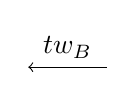
\begin{tikzpicture} \draw[<-] (0,0) -- (1,0); \node at (.5,.25) {$tw_B$}; \end{tikzpicture} &$\sB_{W^T, \s{G^T}}$ \\
%
\begin{tikzpicture} \draw[<->] (0,0) -- (0,1); \end{tikzpicture}& & \begin{tikzpicture} \draw[<->, dashed] (0,0) -- (0,1); \node at (0,1.1) {}; \end{tikzpicture} \\
%
$\sA_{\tw{W},\tw{G}}$ &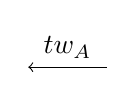
\begin{tikzpicture} \draw[<-] (0,0) -- (1,0); \node at (.5,.25) {$tw_A$};\end{tikzpicture} &$\sA_{W, \s{G}}$ \\
\end{tabular}\end{center}

The two horizontal arrows are the content of Theorem \ref{t:twist} and Corollary \ref{c:Btwistiso}. The dashed arrow is the desired isomorphism of Theorem \ref{t:BViso}. We will establish this map by providing the leftmost vertical arrow in the diagram. This will follow from \cite{Kr} of Krawitz (see Theorem~\ref{t:krawitz}). The only difference is the group of symmetries in the upper left corner is $\tw{(G^T)}$, instead of $\tw{(G)}^T$. Therefore all that remains is to show $\tw{(G^T)} = (\tw{G})^T$, which we do in the following lemma. 
\end{proof}

\begin{lem}
$\tw{(G^T)} = (\tw{G})^T$. 
\end{lem}
\begin{proof}
We first consider the inclusion $\tw{(G^T)}\subset (\tw{G})^T$. Recall $\tw{(G^T)}=(\phi^T)^{-1}(\s{G^T})$. Consider $g=(\alpha, \beta)\in \tw{(G^T)}$ and $g_\epsilon=((1/2)^{\epsilon},\alpha,(1/2)^{\epsilon},\beta)$ for $\epsilon\in\set{0,1}$. By definition, $g_0\in G^T$ or $g_1\in G^T$. 

We want to show that $g\in (\tw{G})^T$, which means we need to show that for each $h=(\gamma_x,\gamma_y)\in \tw{G}$, $gA_{\tw{W}}h\in \ZZ$. Again, $h\in \tw{G}$ means that $h_{\epsilon'}=((1/2)^{\epsilon'},\gamma_x,(1/2)^{\epsilon'},\gamma_y)\in G$ for either $\epsilon'=0$ or $\epsilon'=1$.

Let $A_1$ and $A_2$ be the exponent matrices for $f_1$ and $f_2$, resp. We can compute 
\[
g_\epsilon A_{W}h_{\epsilon'}= 4(1/2)^{\epsilon+\epsilon'}+\alpha A_{1}\gamma_x+\beta A_{2}\gamma_y.
\]
Since the first summand is an integer, we have $gA_{\tw{W}}h=\alpha A_{1}\gamma_x+\beta A_{2}\gamma_y \cong 0 \pmod \ZZ$. 

Now for the reverse inclusion $(\tw{G})^T\subset \tw{(G^T)}$. Suppose $g=(\alpha,\beta)\in (\tw{G})^T$, and again let $g_\epsilon= ((1/2)^{\epsilon},\alpha,(1/2)^{\epsilon},\beta)$. We need to show that either $g_0\in G^T$ or $g_1\in G^T$. In other words we need to show that $g_0A_{W}h\equiv 0\pmod \ZZ$ for every $h\in G$, or that $g_1A_{W}h\equiv 0\pmod \ZZ$ for every $h\in G$. For $h$ of the form $((1/2)^{\epsilon'},\gamma_x,(1/2)^{\epsilon'},\gamma_y)$, the previous calculation shows that this indeed the case for both $g_0$ and $g_1$. The difficulty comes with $h$ is of the form $((1/2)^{\epsilon'},\gamma_x,(1/2)^{1-\epsilon'},\gamma_y)$. We need to differentiate two cases. 

First suppose $\age \alpha\equiv 0 \pmod \ZZ$. Then since $\tw{(G^T)}\subset (\tw{G})^T\subset \SL_{\tw{W}}$, $\age \beta\equiv 0 \pmod \ZZ$. We will show that in fact $g_0\in G^T$. Also notice that $\alpha A_1\jw_x=\age \alpha=0\pmod \ZZ$. For simplicity, suppose $h=((1/2),\gamma_x,0,\gamma_y)$. Then $\jw_{W_1}+h\in \phi(\tw{G})$, and so 
\[
g_0 A_W (\jw_{W_1}+h)=\alpha A_1 \jw_x + \alpha A_1 \gamma_x + \beta A_2 \gamma_y=0\pmod \ZZ.
\]
Hence
\[
g_0 A_W h= \alpha A_1 \gamma_x + \beta A_2 \gamma_y =0\pmod \ZZ.
\]
If $h=(0,\gamma_x,1/2,\gamma_y)$, the proof is the same, only using $\jw_{W_2}$ instead. 

On the other hand suppose $\age \alpha\equiv 1/2 \pmod\ZZ$. Then by similar reasoning also $\age \beta\equiv 1/2 \pmod\ZZ$. We will show that in fact $g_1\in G^T$. The proof is similar, but this time, we notice that $\alpha A_1\jw_x$ is no longer an integer, but a half--integer. Again for simplicity, suppose $h=((1/2),\gamma_x,0,\gamma_y)$. Then $\jw_{W_1}+h\in \phi(\tw{G})$, and so 
\[
g_1 A_W (\jw_{W_1}+h)=\alpha A_1 \jw_x + \alpha A_1 \gamma_x + \beta A_2 \gamma_y\in \ZZ
\]
(because $g\in (\tw{G})^T$). But recall $\alpha A_1\jw_x\equiv \tfrac 12\pmod \ZZ$, hence
\[
g_1 A_W h= \frac 12 + \alpha A_1 \gamma_x + \beta A_2 \gamma_y \in \ZZ.
\]
If $h=(0,\gamma_x,1/2,\gamma_y)$, the proof is the same, only using $\jw_{W_2}$ instead.
\end{proof}

%\cite{Kr}

This concludes the proof of Theorem \ref{t:BViso}. 



\subsection{Landau--Ginzburg Algebra Isomorphism}\label{sec:alg_isom}
We have shown that there is an isomorphism of bi--graded vector spaces. But as we have remarked, each state space also has the structure of a Frobenius algebra over $\CC$. We will now consider the algebra structure. 


\subsubsection{A--model Frobenius algebra}
The product on the A--model is defined in \cite{FJR13} via the structure constants
\[
a\star_{\sA} b:= \sum_{\xi,\xi'}\langle a,b,\xi \rangle_{0,3} \eta^{\xi,\xi'}\xi'
\]
where the sum runs over a basis of $\sA_{W,G}$, and $\eta^{\xi,\xi'}$ are the corresponding entries from the matrix inverse to the pairing matrix $\eta$. 

The structure constants $\langle a,b,\xi \rangle_{0,3}$ are defined in FJRW theory via certain integrals over the moduli space of curves $\overline \cM_{0,3}$, and there are corresponding numbers for higher genus and more marked points as well (see \cite{FJR13}).  Explicit computations of some of these constants in certain cases are given in \cite{FJR13, kpabr, D4, Kr} and most recently in \cite{HLSW}, and methods for computations are given in \cite{Guere, Francis}. 

We will not need these numbers explicitly in this work. We rely instead on the B-model. 


\subsubsection{B-model Frobenius algebra}
On the B--side, the product was defined by Intriligator, Vafa, and Kaufmann \cite{IV, kau1,kau2,kau3}, and written explicitly in the form we will use now by Krawitz \cite{Kr}. It is defined on a basis, and then extended multilinearly to the entire state space. In what follows, we write 
\[
W_{g\cap h}:= W|_{\Fix g \cap \Fix h}
\]
and $\mu_{g\cap h}$ for the dimension of the corresponding Milnor algebra. 

On the basis we have defined, the definition of the product is 

\[
\fjrw{1}{g}\star_{\sB} \fjrw{1}{h} = \gamma_{g,h} \fjrw{1}{gh}, \text{ where}
\]
\[
\gamma_{g,h} \frac{\Hess (W_{g\cap h})}{\mu_{g\cap h}} = \left\{ \begin{array}{l l }
\frac{\Hess (W_{gh})}{\mu_{gh}} & \text{ if } I_g \cup I_h \cup I_{gh} = \{1, \ldots, N\}\\
0 & \text{ otherwise} \\ \end{array}\right.
\]

In \cite{FJJS}, it was shown that for LG models $(W,G)$ satisfying the conditions of Theorem \ref{t:Algiso}, we have an isomorphism of Frobenius algebras
\[
\sA_{W,G}\cong \sB_{W^T,G^T}, 
\]
given by a rescaling of the Krawitz map. 
The conditions are satisfied for a majority of cases---in particular for all polynomials with no chains (see \cite[Remark 1.1.1]{FJJS}). 


\subsubsection{Proof of Theorem~\ref{t:Algiso}}We will now exploit this isomorphism to prove Theorem \ref{t:Algiso}. 

We have the following diagram of Landau--Ginzburg models. The lower vertical (non--dashed) arrows come from Krawitz's mirror map. As mentioned above, under the conditions stated in Theorem \ref{t:Algiso}, there exist rescalings of these maps which are isomorphisms of Frobenius algebras. The horizontal arrows (and vertical double line) are the vector space isomorphisms of the previous section.   

\begin{center}\begin{tabular}{ccc}
$\sB_{\tw{(W^T)},\tw{(G^T)}}$&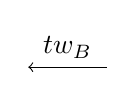
\begin{tikzpicture} \draw[<-] (0,0) -- (1,0); \node at (.5,.25) {$tw_B$}; \end{tikzpicture} &$\sB_{W^T, \s{G^T}}$ \\
%
\begin{tikzpicture} \draw[double] (0,0) -- (0,1); \node at (0,1.1) {}; \end{tikzpicture} & & \begin{tikzpicture} \draw[<->, dashed] (0,0) -- (0,1); \node at (0,1.1) {}; \end{tikzpicture} \\
%
$\sB_{(\tw{W})^T,(\tw{G})^T}$ & &$\sB_{W^T,(\s{G})^T}$\\
%
\begin{tikzpicture} \draw[<-] (0,0) -- (0,1); \node at (.7,1.1) {}; \node at (-.5,.5) {$\kappa_2$}; \end{tikzpicture} & & \begin{tikzpicture} \draw[<-] (0,0) -- (0,1); \node at (-.7,1.1) {}; \node at (.5,.5) {$\kappa_1$};\end{tikzpicture} \\
%
$\sA_{\tw{W},\tw{G}}$&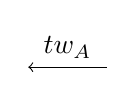
\begin{tikzpicture} \draw[<-] (0,0) -- (1,0); \node at (.5,.25) {$tw_A$};\end{tikzpicture} &$\sA_{W, \s{G}}$ \\
\end{tabular}\end{center}

Using this description as a guide, we will define a map $\varphi:\sB_{W^T,(\s{G})^T} \to \sB_{W^T,\s{G^T}}$, which is closely related (but not equal) to the composition $tw_B^{-1}\circ \kappa_2^{-1} \circ tw_A \circ \kappa_1$ of the solid arrows in the diagram, each of which is a degree--preserving isomorphism of graded vector spaces.  We then show that $\varphi$ preserves products and pairings. The isomorphism of Theorem \ref{t:Algiso} is the composition $\varphi\circ\kappa_1^{-1}$.  



\begin{rem}
It is also worth noting that in the diagram, there are two \emph{different} B--models. This is related to the so--called multiple mirror phenomenon as mentioned in the Introduction. The B--model in the middle of the right-hand side is BHK mirror for $(W,\s{G})$. However, as we have seen, $\s{G^T}\neq (\s{G})^T$ and so the corresponding geometry does not fit the Borcea--Voisin construction. Because of the LG/CY correspondence, we expect a B--model whose corresponding geomoetry is Borcea--Voisin type, which is what the upper right--hand B--model is. Also, since we have two B models, both mirror to the same A model, it should be expected that the two B model state spaces are isomorphic. 
\end{rem}

For the proof of Theorem \ref{t:Algiso}, we introduce the notation $\sB_1 = \sB_{W^T, (\s{G})^T}$ (the BHK mirror) and $\sB_2 = \sB_{W^T, \s{G^T}}$ (the BV mirror). 


%%%%%%%%%%%%%%%%%%%%%%%%%%%%%%%%%%%
\iffalse
\nathanin{I suggest we leave out the next computations in the final draft. They are good for now to check the math, but in the final draft, I suggest we simply say what $\sB_1$ and $\sB_2$ are, and then give the map $\varphi$.}
\textit{Notation}:  We will use the notation $\rho^x_i$ to denote the column of $A_{W}^{-1}$ corresponding to $x_i$, $\rho^y_j$ for that corresponding to $y_j$, ($\mathring{\rho}^x_i$, $\mathring{\rho}^y_j$ for the corresponding columns of $A_{\tw{W}}^{-1}$)  and $\tilde{\rho}^x_k$ and $\tilde{\rho}^y_\ell$ ($\mathring{\tilde{\rho}}^x_i$, $\mathring{\tilde{\rho}}^y_j$) for the corresponding rows, respectively. 
\amandain{I'm not in love with this notation....}

Let $\fjrw{m}{g}$ be a generator in $\sB_{W^T, (\s{G})^T}$.  Let $I = I_x \cup I_y$ be the set of indices fixed by $g$. Write $m = \prod_{i \in I_x} x^{a^x_i} dx_i \prod_{j \in I_y} y^{a^y_j} dy_j$, and set 
\[
g^A = \sum_{i \in I_x} \rho^x_i(a^x_i+1)+ \sum_{j \in I_y} \rho^y_j(a^y_j+1)
\]
 Let $J = J_x \cup J_y$ be the set of indices fixed by $g^A$.  We can now write 
 \[
 g = \sum_{k\in J_x} \tilde{\rho}^x_k(r^x_k+1)+ \sum_{\ell \in J_y} \tilde{\rho}^y_\ell(r^y_\ell+1),
 \]
 and these $r_i$'s satisfy bounds set out by Krawitz.  Set 
 \[
 m^A = \prod_{k \in J_x} x_k^{r_k}dx_k \prod_{\ell \in J_y} y_\ell^{s_\ell}dy_\ell.
 \]
Thus $\kappa_1(\fjrw{m}{g})=c_1 \fjrw{m^A}{g^A}$, for some scalar $c_1$\nathan{Is this not 1?}. 

Now we apply the twist map.  If 
\[
(m^A)' = \prod_{k \in J_x \setminus \{0_x\}} x_k^{r_k}dx_k \prod_{\ell \in J_y \setminus \{0_y\}} y_\ell^{s_\ell}dy_\ell,
\]  
 and 
 \[
 (g^A)' = \sum_{i \in (I_x\setminus 0)} \mathring\rho^x_i(a^x_i+1)+ \sum_{j \in (I_y \setminus 0)} \mathring\rho^y_j(a^y_j+1)
 \]
 We have
  $tw_A \kappa_1 (\fjrw{m}{g}) = c_1 \cdot c_2 \fjrw{(m^A)'}{(g^A)'}$.
  
  

Now we take the inverse of the mirror map on the twisted side.   It is clear that $\tilde{J} = J \setminus \{0_x, 0_y\}$ is the set of indices fixed by $(g^A)'$ (since these correspond to the volume forms of $(m^A)'$).  Write 
\[
h' =  \sum_{k \in (J_x\setminus 0)} \mathring{\tilde{\rho}}^x_k(r^x_k+1)+ \sum_{\ell \in (J_y \setminus 0)} \mathring{\tilde{\rho}}^y_\ell(s^y_\ell+1).
\]
Notice that the only rows of $A^{-1}$ that are excluded in $h'$ are those corresponding to $x_0$ and $y_0$, and those columns have entries only in the $x_0$ and $y_0$ positions.  Thus, the indices fixed by $h'$ are exactly those (excluding $x_0$ and $y_0$) in $I$. In fact, we used this set of indices to obtain $(g^A)'$, which gives us the mirror monomial: 
\[
n' =   \prod_{i \in (I_x\setminus 0)} x_i^{a^x_i}dx_i \prod_{j \in (I_y \setminus 0)} y_j^{a^y_j}dy_j
\]
  
At this point we have determined that $ \kappa_2^{-1} tw_A \kappa_1 (\fjrw{m}{g}) = c_1 \cdot c_2\cdot c_3 \fjrw{n'}{h'}$

Finally, we take the inverse of the twist map on the B--side.  The group element $h' = (\alpha, \beta)$ (where $\alpha$ acts on the variables $x_1, \ldots, x_m$ and $\beta$ acts on the variables $y_1, \ldots, y_n$) must be sent $(\epsilon/2, \alpha, \epsilon/2, \beta)$, where $\epsilon \in \{0,1\}$ depends on the action of $\jw_x$ on $(n')_x$.  Say 
\[
h' \mapsto \sum_{k \in (J_x\setminus 0)} \tilde{\rho}^x_k(r^x_k+1)+ \sum_{\ell \in (J_y \setminus 0)} \tilde{\rho}^y_\ell(s^y_\ell+1) + \epsilon(\tilde{\rho}^x_0 +  \tilde{\rho}^y_0), \text{ and }
\]

\[
n' \mapsto \epsilon n' + (1-\epsilon)n'\wedge dx_0\wedge dy_0
\]  
Where $\epsilon =0$ if If $\jw_x$  acts with weight zero on $(n')_x$, and $\epsilon = 1$ otherwise.

\nathanin{I would suggest we leave out from the last comment until here. See above.}
\fi
%%%%%%%%%%%%%%%%%%%%%%%%%%%%%%%%%%%%%%%%%%%%%

As suggested by the composition $tw_B^{-1}\circ \kappa_2^{-1} \circ tw_A \circ \kappa_1$, the map $\varphi$ should have the following form for some nonzero constant $\kappa_{m,g}$: 

\[
\varphi(\fjrw{m}{g})= \left\{ \begin{array}{ll}
\kappa_{m,g}\fjrw{m}{g} &  \text{ if }\jw_x\text{ acts with weight 0 on }m_x,\\
 \kappa_{m,g}\fjrw{\tilde{m}}{\sigma{g}} & \text{ otherwise}, \end{array}\right.
 \]
where $\tilde{m}$ differs from $m$ by the $dx_0\wedge dy_0$ volume form. That is to say. if $m$ has $dx_0\wedge dy_0$, then $\tilde{m}$ does not, and vice-versa. This is a degree preserving bijection between B--models.  

All that remains is to give the constants $\kappa_{m,g}$, which we do as follows: 
\[
\varphi(\fjrw{m}{g}) = \left\{ \begin{array}{ll} \fjrw{m}{g} & \text{if } \fjrw{m}{g} \in \sB_{W^T, \s{G^T}} \\ 
\tfrac 12 \fjrw{\tilde m}{\sigma g} & \text{if } \fjrw{m}{g} \notin \sB_{W^T, \s{G^T}}, g = (0, \alpha, 0, \beta) \\ 
2\fjrw{\tilde m}{\sigma g} & \text{if } \fjrw{m}{g} \notin \sB_{W^T, \s{G^T}}, g = (1/2, \alpha, 1/2, \beta). \\ 
\end{array}\right.
\]

In other words, $\kappa_{m,g} =1$ if $ \fjrw{m}{g} \in \sB_{W^T, \s{G^T}}$ and $\kappa_{m,g}\in \{1/2,2\}$ otherwise. Since the dependence on $m$ only determines if $\kappa_{m,g}=1$ or not, we can henceforth drop the subscript $g$ with no confusion, i.e. $\kappa_g=\kappa_{m,g}$. 

We make the following two useful remarks to characterize whether $\fjrw{m}{g}\in \sB_{W^T,\s{G^T}}$. 
%\begin{rem}\label{rem_wts_contain}
For $\fjrw{m}{g}\in \sB_1$, we see that $g$ is always an element of $\s{G^T}$, since $(\s{G})^T\subset \s{G^T}$. But $m$ may not be fixed by the action of all elements in the larger group. One can show that $\jw_{W_1^T}$ fixing $m_x$ is equivalent to saying that $\fjrw{m}{g} \in \sB_2=\sB_{W^T, \s{G^T}}$. Recall that $J_{W_1^T}\times J_{W_2^T}\subset \s{G^T}$. \nathan{Amanda wanted to fix this part up a bit, and check the computations. The computations are still in code prior to this discussion.}
%\end{rem}

%\begin{rem}\label{rem_action}
Notice that if $\fjrw{m}{g}$ and $\fjrw{n}{h}$ are elements in $\sB_1$, and $m_x$ and $n_x$ are fixed by $\jw_x$ in $\sB_2$, then $(mn)_x$ is also fixed. On the other hand, if the action on both $m_x$ and $n_x$ is with weight 1/2, then $(mn)_x$ is fixed.  Only if one is fixed, and the action on the other is with weight $1/2$ and the action on the product is with weight $1/2$. 
%\end{rem}

\begin{lem} The map $\varphi$ preserves products.
\end{lem}
  
\begin{proof}
%First recall that B--model products are defined on the algebra generators in the following way: 
%\[
%\fjrw{1}{g}\star_{\sB} \fjrw{1}{h} = \gamma_{g,h} \fjrw{1}{gh}, \text{ where}
%\]
%\[
%\gamma_{g,h} \frac{\Hess (W_{g\cap h})}{\mu_g \cap\mu_h} = \left\{ \begin{array}{l l }
%\frac{\Hess (W_{\Fix(gh)})}{\mu_{gh}} & \text{ if } I_g \cup I_h \cup I_{gh} = \{1, \ldots, N\}\\
%0 & \text{ otherwise} \\ \end{array}\right.
%\]
Based on the definition of $\varphi$, there are several cases to check. 

\noindent \textbf{Case A:} Suppose that $\fjrw{m}{g}$ and $\fjrw{n}{h}$ are each elements of both $\sB_1$
and $\sB_2$. Based on the previous remarks, $\fjrw{mn}{gh}$ is in both as well, and so 
\[
\begin{array}{l}
\varphi(\fjrw{m}{g} \star_1 \fjrw{n}{h}) = \varphi( \gamma_{g,h} \fjrw{mn}{gh}) = \gamma_{g,h} \fjrw{mn}{gh} \\
=
\fjrw{m}{g} \star_2 \fjrw{n}{h}=\varphi(\fjrw{m}{g}) \star_2 \varphi(\fjrw{n}{h})
\end{array}
\]

\noindent \textbf{Case B:} Next, suppose that $\fjrw{m}{g}$ and $\fjrw{n}{h}$ are each elements of $\sB_1$, but neither are elements of $\sB_2$.   
Notice that in this case 
\[
\varphi(\fjrw{m}{g}) \star_2 \varphi(\fjrw{ n}{ h})=k_g\fjrw{\tilde m}{\sigma g} \star_2 k_h\fjrw{\tilde n}{\sigma h} = k_gk_h\gamma_{\sigma g, \sigma h} \fjrw{mn}{ gh},
\]
since $\sigma g \sigma h = gh$.  Further, $\varphi( \fjrw{mn}{ gh}) = \fjrw{mn}{ gh}$, by Remark \ref{rem_action}. Thus, to verify that  
$
\varphi(\fjrw{m}{ g}) \star_2  \varphi( \fjrw{n}{ h}) =\varphi(\fjrw{m}{ g} \star_1   \fjrw{n}{ h})$, % =  \varphi(\gamma_{ g, h} \fjrw{mn}{ gh})\\
%\fjrw{\tilde m}{\sigma g} \star_2 \fjrw{\tilde n}{\sigma h} = 
we only need to check that 
\[
k_gk_h\gamma_{\sigma g, \sigma h} \fjrw{mn}{gh}= \gamma_{g, h} \fjrw{mn}{ gh}.
\]


There are three relevant cases. 
\begin{enumerate}
\item $g$ and $h$ are both of the form $(0, \alpha, 0, \beta)$
\item $g$ and $h$ are both of the form $(1/2, \alpha, 1/2, \beta)$
\item $g$ is of one of the above forms and $h$ is of the other.
\end{enumerate}

It is straightforward to verify that in each case, 
$I_g \cup I_h \cup I_{gh} = \{x_0, \ldots, x_m,y_0,\ldots,y_n\}$
 if and only if 
$I_{\sigma g} \cup I_{\sigma h} \cup I_{gh} = \{x_0, \ldots, x_m,y_0,\ldots,y_n\}$.


We verify the details of the preservation of the product in only the first case; the others follow by similar arguments. 
\begin{enumerate}
\item  $g$ and $h$ are both of the form $(0, \alpha, 0, \beta)$. \\
Here, $k_g = k_h = 1/2$. Suppose that $I_g \cup I_h \cup I_{gh} = \{x_0, \ldots, x_m,y_0,\ldots,y_n\}$. Then, 
\[
\gamma_{g,h}  =
\frac{\Hess (W_{gh})\mu_{g \cap h}}{\Hess (W_{g\cap h})\mu_{gh}} 
=\frac{\Hess (W_{gh})\mu_{\sigma g \cap \sigma h}}{4\Hess (W_{\Fix(\sigma g)\cap \Fix(\sigma h)})\mu_{gh}} 
=\tfrac 14  \gamma_{\sigma g,\sigma h}
\]

So, we have, $k_gk_h\gamma_{\sigma g, \sigma h} = 1/4 \cdot \gamma_{\sigma g,\sigma h} = \gamma_{g,h}$, as desired. 
\iffalse
\amandain{Maybe we don't need to show every detail here.  Similarly, the other cases...}

\item  $g$ and $h$ are both of the form $(1/2, \alpha, 1/2, \beta)$.\\
Here, $k_g = k_h = 2$. Again, suppose that $I_g \cup I_h \cup I_{gh} = \{x_0, \ldots, x_m,y_0,\ldots,y_n\}$. Then, 
\[
1/4\gamma_{g,h}  =
\frac{\Hess (W_{gh})\mu_{g \cap h}}{4\Hess (W_{g\cap h})\mu_{gh}} 
=\frac{\Hess (W_{gh})\mu_{\sigma g \cap \sigma h}}{\Hess (W_{\Fix(\sigma g)\cap \Fix(\sigma h)})\mu_{gh}} 
=  \gamma_{\sigma g,\sigma h}
\]

So, we have, $k_gk_h\gamma_{\sigma g, \sigma h} = 4 \cdot \gamma_{\sigma g,\sigma h} = \gamma_{g,h}$, as desired. 


\item  $g$ is of one of the above forms and $h$ is of the other. \\
Here, $k_g =1/2,  k_h = 2$. Again, suppose that $I_g \cup I_h \cup I_{gh} = \{x_0, \ldots, x_m,y_0,\ldots,y_n\}$. Then, 
\[
\gamma_{g,h}  =
\frac{\Hess (W_{gh})\mu_{g \cap h}}{\Hess (W_{g\cap h})\mu_{gh}} 
=\frac{\Hess (W_{gh})\mu_{\sigma g \cap \sigma h}}{\Hess (W_{\Fix(\sigma g)\cap \Fix(\sigma h)})\mu_{gh}} 
=  \gamma_{\sigma g,\sigma h}
\]

So, we have, $k_gk_h\gamma_{\sigma g, \sigma h} = 2 \cdot 1/2 \cdot \gamma_{\sigma g,\sigma h} = \gamma_{g,h}$, as desired. 

\fi
\end{enumerate}


\noindent \textbf{Case C:} Finally, we must consider the case when $\fjrw{m}{g}, \fjrw{n}{h}$ are both elements of $\sB_1$, but only one of them is an element of $\sB_2$.  Without loss of generality, we say $\fjrw{m}{g} \in \sB_2$.  Notice that in this case
\[
\varphi(\fjrw{m}{g} \star_{\sB_1} \fjrw{n}{h}) = \varphi(\gamma_{g,h} \fjrw{mn}{gh}) = \gamma_{g,h}k_{gh} \fjrw{mn} {\sigma gh},
\]
by Remark \ref{rem_action}. Additionally, 
\[
\varphi(\fjrw{m}{g}) \star_{\sB_2} \varphi(\fjrw{n}{h}) = \fjrw{m}{g} \star_{\sB_2} k_h \fjrw{n}{\sigma h} = \gamma_{g,\sigma h}k_{h} \fjrw{mn} {\sigma gh}.
\]
We must prove $\gamma_{g,h}k_{gh} \fjrw{mn} {\sigma gh} =\gamma_{g,\sigma h}k_{h} \fjrw{mn} {\sigma gh}$ in  the following  four cases: 
\begin{enumerate}
\item $g$ and $h$ are both of the form $(0, \alpha, 0, \beta)$ ($k_h =k_{gh}= 1/2$)
\item $g$ and $h$ are both of the form $(1/2, \alpha, 1/2, \beta)$ ($k_h = 2, k_{gh}= 1/2$).
\item $g$ is of the form $(0, \alpha, 0, \beta)$, and $h$ is of the form $(1/2, \alpha, 1/2, \beta)$ ($k_h = k_{gh}= 2$)
\item $g$ is of the form $(1/2, \alpha, 1/2, \beta)$, and $h$ is of the form $(0, \alpha, 0, \beta)$ ($k_h= 1/2,  k_{gh}= 2$).
\end{enumerate}

Again, we verify the preservation of the product in the first case only; the others follow similarly. 
\begin{enumerate}
\item $g$ and $h$ are both of the form $(0, \alpha, 0, \beta)$ ($k_h =k_{gh}= 1/2$)\\
\[
\gamma_{g,h}  =
\frac{\Hess (W_{gh})\mu_{g \cap h}}{\Hess (W_{g\cap h})\mu_{gh}} 
=\frac{4 \Hess (W_{\sigma gh})\mu_{ g \cap \sigma h}}{4\Hess (W_{\Fix( g)\cap \Fix(\sigma h)})\mu_{\sigma gh}} 
=  \gamma_{g,\sigma h}
\]
So, 
$k_{gh}\gamma_{g,h} = \tfrac 12 \gamma_{g,h} = \tfrac 12 \gamma_{g,\sigma h} = k_{h}\gamma_{g,\sigma h}$, as desired. 
\iffalse

\amandain{Maybe we don't need to show every detail here.  Similarly, the other cases...}
\item $g$ and $h$ are both of the form $(1/2, \alpha, 1/2, \beta)$ ($k_h = 2, k_{gh}= 1/2$).
\[
\gamma_{g,h}  =
\frac{\Hess (W_{gh})\mu_{g \cap h}}{\Hess (W_{g\cap h})\mu_{gh}} 
=\frac{4\Hess (W_{\sigma gh})\mu_{ g \cap \sigma h}}{\Hess (W_{\Fix( g)\cap \Fix(\sigma h)})\mu_{\sigma gh}} 
=  4\gamma_{g,\sigma h}
\]
So, 
$k_{gh}\gamma_{g,h} = 1/2 \gamma_{g,h} = 2\gamma_{g,\sigma h} = k_{h}\gamma_{g,\sigma h}$, as desired. 


\item $g$ is of the form $(0, \alpha, 0, \beta)$, and $h$ is of the form $(1/2, \alpha, 1/2, \beta)$ ($k_h = k_{gh}= 2$).

\[
\gamma_{g,h}  =
\frac{\Hess (W_{gh})\mu_{g \cap h}}{\Hess (W_{g\cap h})\mu_{gh}} 
=\frac{1/4 \Hess (W_{\sigma gh})\mu_{ g \cap \sigma h}}{1/4 \Hess (W_{\Fix( g)\cap \Fix(\sigma h)})\mu_{\sigma gh}} 
=  \gamma_{g,\sigma h}
\]
So, 
$k_{gh}\gamma_{g,h} = 2 \gamma_{g,h} = 2\gamma_{g,\sigma h} = k_{h}\gamma_{g,\sigma h}$, as desired. 

\item $g$ is of the form $(1/2, \alpha, 1/2, \beta)$, and $h$ is of the form $(0, \alpha, 0, \beta)$ ($k_h= 1/2,  k_{gh}= 2$).

\[
\gamma_{g,h}  =
\frac{\Hess (W_{gh})\mu_{g \cap h}}{\Hess (W_{g\cap h})\mu_{gh}} 
=\frac{1/4\Hess (W_{\sigma gh})\mu_{ g \cap \sigma h}}{\Hess (W_{\Fix( g)\cap \Fix(\sigma h)})\mu_{\sigma gh}} 
=  1/4\gamma_{g,\sigma h}
\]
So, 
$k_{gh}\gamma_{g,h} = 2 \gamma_{g,h} = 1/2\gamma_{g,\sigma h} = k_{h}\gamma_{g,\sigma h}$, as desired. 
\fi
\end{enumerate}
 
\end{proof}

\begin{rem}
Recall that the for an element $\fjrw{m}{g}$ from an LG state space, $m$ represents a monomial together with a volume form.  In the following proof, we are sometimes interested in only the monomial portion of $m$ (which by abuse of notation, we will call $m$).  Further, we point out that the monomial portion of both $m$ and $\tilde{m}$ are the same. 
\end{rem}

\begin{lem}The map $\varphi$ preserves the pairing. 
\end{lem}


\begin{proof}
Recall that if $\langle \fjrw{m}{g}, \fjrw{n}{g^{-1}}\rangle_{\sB_1} \neq 0$, then we have 
\[
mn = \frac{\langle \fjrw{m}{g}, \fjrw{n}{g^{-1}}\rangle_{\sB_1}}{\mu_g}\Hess(W_g) + l.o.t
\]
 If both $\fjrw{m}{g}$ and  $\fjrw{n}{g^{-1}}$ are in $\sB_2$, then the pairings are computed in exactly the same way in both $\sB_1$ and $\sB_2$ 

If neither $\fjrw{m}{g}$ nor $\fjrw{n}{g^{-1}}$ are in $\sB_2$, then we have two cases to consider. 
\begin{enumerate}
\item $g$ is of the form $(0, \alpha, 0, \beta)$. \\
\[
m \cdot n = \frac{\langle \fjrw{m}{g}, \fjrw{n}{g^{-1}} \rangle_{\sB_1}}{\mu_g} \Hess(W_g)  = \frac{\langle \fjrw{m}{g}, \fjrw{n}{g^{-1}} \rangle_{\sB_1}}{\mu_{\sigma g}} 4 \Hess(W_{\sigma g}) 
\]
Thus, for $\varphi(\fjrw{m}{g}) = \tfrac 12 \fjrw{\tilde m}{\sigma g}$, and  $\varphi(\fjrw{n}{g^{-1}}) = \tfrac 12 \fjrw{\tilde n}{\sigma g^{-1}}$
\[
 \tfrac 12 m \cdot \tfrac 12 n   = \frac{\langle \fjrw{m}{g}, \fjrw{n}{g^{-1}} \rangle_{\sB_1}}{\mu_{\sigma g}}  \Hess(W_{\sigma g}). 
\]
So, $ \langle \fjrw{m}{g}, \fjrw{n}{g^{-1}} \rangle_{\sB_1} = \langle \varphi(\fjrw{m}{g}), \varphi(\fjrw{n}{g^{-1}}) \rangle_{\sB_2}$.

\item $g$ is of the form $(1/2, \alpha, 1/2, \beta)$. \\
\[
m \cdot n = \frac{\langle \fjrw{m}{g}, \fjrw{n}{g^{-1}} \rangle_{\sB_1}}{\mu_g} \Hess(W_g)  = \frac{\langle \fjrw{m}{g}, \fjrw{n}{g^{-1}} \rangle_{\sB_1}}{\mu_{\sigma g}} \tfrac 14 \Hess(W_{\sigma g}) 
\]
Thus, for $\varphi(\fjrw{m}{g}) = 2\fjrw{\tilde m}{\sigma g}$, and  $\varphi(\fjrw{n}{g^{-1}}) = 2\fjrw{\tilde n}{\sigma g^{-1}}$
\[
2m \cdot 2n   = \frac{\langle \fjrw{m}{g}, \fjrw{n}{g^{-1}} \rangle_{\sB_1}}{\mu_{\sigma g}}  \Hess(W_{\sigma g}). 
\]
So, $ \langle \fjrw{m}{g}, \fjrw{n}{g^{-1}} \rangle_{\sB_1} = \langle \varphi(\fjrw{m}{g}), \varphi(\fjrw{n}{g^{-1}}) \rangle_{\sB_2}$.
\end{enumerate}

Note that if $\fjrw{m}{g}$ is in $\sB_2$ but  $\fjrw{n}{g^{-1}}$ is not, then $\langle\fjrw{m}{g},\fjrw{n}{g^{-1}}\rangle=0$, since the $\jw_x$ acts with weight zero on the Hessian. Thus, we have verified that $\varphi$ preserves both the product and the pairing, and therefore, the composition, $\varphi \circ \kappa_1^{-1}$ is an isomorphism of Frobenius algebras. (When Property $\star$ of \cite{FJJS} is satisfied). 

\end{proof}



%We also need to show that the change of degrees is the same on the top as on the bottom. This would finish the proof of the theorem. 


\section{A Geometric View}\label{s:geometry}

In this section, we consider the geometry of the Borcea--Voisin model. We begin by describing a construction called the GLSM, which gives some reason why we expect the LG/CY correspondence to hold. % the basis for the LG/CY correspondence. %This justifies the terminology BVLG model. 
In Section~\ref{ss:LGCYstatespace} we will describe the LG/CY state space isomorphism, establishing an equivalence between the BVLG model state space and the state space of the BV orbifold. In Section~\ref{ss:twistmap} we describe the twist map on the geometric side, generalizing the twist map of \cite{Borcea} and \cite{ABS}. In Section~\ref{ss:applications} we pull everything together and discuss some consquences in the corresponding geometry. 



\subsection{Gauged linear sigma models}\label{ss:GLSM}
We include this section, in order to demonstrate why the LG model described in Section~\ref{ss:BVLGmodel} has the particular form we have described there. None of the ideas presented in this section will be used in any later proofs. 

The LG/CY correspondence is part of a larger idea due to Ed Witten, in which he considers each theory in the correpondence (e.g. GW theory or FJRW theory) as different ``phases'' of some larger theory called the \emph{gauged linear sigma model} (GLSM) that depends on a parameter. Variation of this parameter will then produce the various theories involved in the LG/CY correspondence. The different phases of the GLSM are conjectured to be equivalent to each other in some certain sense. The first evidence of this equivalence is an isomorphism of the respective state spaces in each phase. 

These ideas have recently been mathematically formalised by Fan--Jarvis--Ruan in \cite{FJR15} and we begin this section by briefly describing their construction. We are intentionally vague about some aspects of this construction, since they are not necessary for our purposes. In this article, we are primarily interested in the state spaces, so we will focus our attention there. 

A GLSM depends on a choice of (1) a finite dimensional vector space $V$ over $\CC$, (2) a reductive algebraic group $G_V$ acting on $V$, (3) a $G_V$--character $\theta$, and (4) a \emph{superpotential} $\overline W: V\to \CC$. From these ingredients, one obtains a \emph{state space}, a \emph{moduli space of LG--quasimaps} with a good virtual cycle, and numerical invariants defined as integrals over the virtual cycle.\nathan{I restructured this. The text is more dense now, but also a quicker read. What do you think? We could make list out of the input still, if it would make it look better there.}
%\begin{itemize}
%	\item a finite dimensional vector space $V$ over $\CC$;
%	\item a reductive algebraic group $G_V\subset \GL(V)$;
%	\item a $G$--character $\theta$ with the property that the semi--stable locus in $V$ coincides with the stable locus, i.e. $V_G^{ss}(\theta)=V_G^{s}(\theta)$--- we denote the corresponding GIT (orbifold) quotient $\cX_\theta=[V\git_\theta G_V]$;
%	\item a choice of $\CC^*$ action ($R$--charge) on $V$ compatible with $G$, which will be denoted by $\CC^*_R$. From this we define $\Gamma=G_V\CC^*_R$;
%	\item a \emph{superpotential} $\overline W: V\to \CC$ of degree $d$ with respect to the $\CC_R^*$ action, such that the GIT quotient of the critical locus is compact;
%	\item a stability parameter $\epsilon>0$;
%	\item and a $\Gamma$ character $\vartheta$ that defines a \emph{good lift} of $\theta$. 
%\end{itemize}

%With the above data, one obtains the following objects:
%\begin{itemize}
%	\item a \emph{state space}, which is the relative Chen--Ruan cohomology of the quotient $\cX_\theta$ with an additional shift in grading,
%	\item a \emph{moduli space of LG--quasimaps},
%	\item a good virtual cycle, 
%	\item numerical invariants, defined as integrals over the virtual cycle. 
%\end{itemize}

If we vary the character $\theta$, we get a different GIT quotient, and therefore a different theory. We can vary the character in the so--called phase space. This space of characters is partitioned into various chambers. Varying the character within a chamber, does not change the theory. However, if we cross into a different chamber, we obtain a different theory. 

The idea behind the LG/CY correspondence is that if we choose the character $\theta$ in a certain chamber, we obtain GW theory of a particular orbifold, whereas if we choose the character in different chamber, we should expect to obtain FJRW theory. 
The moduli space, virtual cycle and numerical invariants from the GLSM will give rise to such structures for Gromov--Witten theory and for FJRW theory. It has conjectured that these structures will agree in some sense  for both theories, but as mentioned we will focus our attention on the state spaces. 

%\nathan{We could actually drop the definition of the state spaces here, if we don't want to mess with the Thom isomorphism.} 
%In order to define the state space, we define for each conjugacy classes $\Psi$ of $G$ for which the fixed locus $\cX_{\theta,\Psi}$ of $\theta$ is non--empty the vector space
%\[
%\sH_{\Psi}=H^{*+2q}(\cX_{\theta,\Psi}, W^\infty, \QQ).
%\]
%The state space is then defined as 
%\[
%\sH_{W,G}=\sum_{\Psi}\sH_\Psi
%\]
%where the sum runs over all conjugacy classes of $G$. 

%As one can see from the input data, there are several parameters which one might vary, to obtain a potentially different theory. In particular, 
%If we vary the character of $G$, we get a different GIT quotient, and therefore a different theory. The idea behind the LG/CY correspondence is that if we vary the character $\theta$, we obtain GW theory of a particular orbifold in one phase, whereas in another phase we should expect to find FJRW theory. 

The relevant GLSM's for BV models are obtained using the following input. Let $V=\CC^{n+m+2}\times \CC^2$ with coordinates $x_0,\dots,x_n,y_0,\dots,y_m$ and $p_1,p_2$. Next we define an action of $(\CC^*)^2$ on $V$ via the weights
\[
\left(\begin{matrix}
u_0 & \dots & u_n & 0 & \dots & 0 & -d_1 & 0\\
0 & \dots & 0 & v_0 & \dots & v_m & 0 & -d_2  
\end{matrix}
\right)
\]
We can embed $(\CC^*)^2$ as diagonal matrices into $\GL(V)$ via these weights.

We can similarly embed the group $G_{max}\hookrightarrow \GL(V)$ acting only on the $x$ and $y$ coordinates. Our reductive group $G_V$ we define as the subgroup of $\GL(V)$ generated by $(\CC^*)^2$ and $\s{G}$. 
For a superpotential, we take $\overline{W}=p_1W_1 + p_2W_2$. %For $R$--charge, we let $\CC^*_R$ act only on the $p$ variables with weight 1.

In order to describe the two relevant GIT quotients, we need to choose appropriate characters of $G_V$. In order to identify the characters, we use the method of symplectic reduction. For more on this perspective and the relationship between symplectic reduction and GIT quotients, see the original construction on GLSM by Fan--Jarvis--Ruan \cite{FJR15}. We take the standard K\"ahler metric on $V$. Since $G_V$ is reductive, it is the complexification of a maximal compact Lie subgroup $H$ acting on $V$ via a faithful unitary representation. The Lie algebra in our case is $\RR^2$. 

We consider the Hamiltonian action of $H$ on $V$, which has moment map $\mu:V\to \RR^2$ given by 
\[
\mu_1 = \sum_{i=0}^n u_i|x_i|^2 - d_1|p_1|^2, \quad \mu_2 = \sum_{j=0}^m v_i|y_i|^2 - d_2|p_2|^2.
\]
The set of critical values for this moment map is $\set{\tau_1=0}\cup\set{\tau_2=0}\subset \RR^2$.

The conditions for the appropriate GIT quotients translate to the requirement of having a regular value of the moment map in the symplectic setting. Once we have our regular values we can return the the algebraic setting to describe the GIT quotients.  Notice the set of critical values divides $\RR^2$ into 4 chambers. Each regular value withing a given chamber will yield an isomorphic GIT quotient. 

A the derivation of a character defines a weight in the Lie algebra $\RR^2$. We will now discuss the two chambers which yield GW theory and FJRW theory. We  will first describe the regular values which yield the relevant characters. Then we will return the the GIT perspective, and describe the unstable locus and the corresponding GIT quotient for each character which has derivation in the given chamber. 

%In order to describe the two relevant GIT quotients, we use the method of symplectic reduction, which as can be shown yields a quotient isomorphic to the GIT quotient (cf. e.g. \cite{FJR13}). In general, given a symplectic manifold $M$ endowed with a Poisson action of a connected Lie group $\cG$ (that is, an action which sets up a skew--product isomorphism between $C^{\infty}(M)$ and the corresponding Lie algebra $\mathfrak{g}$), one may consider the \textit{moment map} $\mu:M \to \mathfrak{g}^*$. % given by $\mu: p \mapsto \mu_X(m)$. 
%Then we define $M//\cG := \mu^{-1}(x)/\cG$ for a regular value $x\in \mathfrak{g}^*$. Here $x$ being a regular value corresponds to taking a character $\theta$ satisfying the semisimplicity condition defined earlier. %This GIT quotient is then endowed with a unique symplectic form induced from the projection from $M_0$ to $\tilde{M}$ and the inclusion map $M_0 \hookrightarrow M$. %\nathan{Add a quick description of symplectic reduction.} \andrew{Very quick. Suffices?} 

%In our case, the group $G_V$ is not connected, so we consider the orbifold
%\[
%\left[\Big(\mu^{-1}(x)\git(\CC^*)^2\Big)/\widetilde{\s{G}}\right].
%\] 
%abelian, since the action of every group element is diagonal. 


\subsubsection*{GW phase} The first chamber we consider is defined by $\tau_1>0, \tau_2>0$. In this chamber, the unstable locus is the set of points in $\CC^{n+m+2}$ with $(x_0,\dots,x_n)\neq 0$, and $(y_0,\dots,y_m)\neq 0$. We get as a GIT quotient 
\[
\left[(\CC^{n+1}\setminus 0)\times (\CC^{m+1}\setminus 0)\times \CC^2/G_V\right]\cong \left[\cO_{\PP(u_0,\dots,u_n)}(-d_1)\times \cO_{\PP(v_0,\dots,v_n)}(-d_2)/\widetilde{\s{G}}\right],%\to \PP(u_0,\dots,u_n)\times \PP(u_0,\dots,n_n). 
\]
Here $\widetilde{\s{G}}=\s{G}/(J_1\times J_2)$. The critical locus of $\overline{W}$ is $\set{W_1=0,W_2=0, p_1=p_2=0}/\widetilde{\s{G}}$, which is the stack 
\[
\left[X_{W_1}\times X_{W_2}/\widetilde{\s{G}} \right].
\]
If we set $n=2, m=3$ this has a Borcea--Voisin variety as crepant resolution. Though it has not been verified in every case, the state space corresponding corresponding to this GIT quotient is expected to be the Chen--Ruan cohomology of the critical locus of $\overline{W}$. In the next section, we will show that the Chen--Ruan cohomology of the Borcea--Voisin orbifold is indeed isomorphic to the state space of FJRW theory.   



\subsubsection*{FJRW phase} The other relevant chamber is defined by $\tau_1<0, \tau_2<0$. The unstable locus the set of points in $V$ with $p_1\neq 0$, and $p_2\neq 0$. We get the GIT quotient 
\[
\left[\CC^{n+m+2}\times (\CC^*)^2/G_V\right]\cong [\CC^{n+m+2}/\s{G}] 
\]
With superpotential $\overline{W}=W$ (we scaled away the $p$'s).

The critical locus of $\overline{W}$ is the origin. In this chamber, the state space is exactly the state space of FJRW theory.   

Because both theories are merely different phases of the same GLSM, we expect the theories to be equivalent. The most basic manifestation of this equivalence is an isomorphism of state spaces, which we show in the next section.    




\subsection{LG/CY correspondence: state space isomorphism}\label{ss:LGCYstatespace}

In this section, we will prove that the two state spaces described above are isomorphic as graded vector spaces, i.e. 
\begin{equation}\label{e:stateiso}
\sA_{W,\s{G}}^{p,q}\cong H_{CR}^{p,q}\Big(\big[X_{W_1}\times X_{W_2}/\widetilde{\s{G}} \big];\CC\Big) 
\end{equation}
This is similar to what was done by Chiodo--Ruan in \cite{ChR}. However, there are some important differences, so we will give the details here. 
We begin by expressing each side of Equation~\eqref{e:stateiso} in a more useable form. 



\subsubsection{FJRW state space} 
We begin with FJRW theory. 
In order to simplify notation, we will write $J=J_1\times J_2$. For $g\in \s{G}$, we write $g=(g_1,g_2)$ with $g_1\in G_{W_1}^{max}$ and $g_2\in G_{W_2}^{max}$. Notice this differs slightly from previous sections, where we wrote $g=(\epsilon/2,\alpha,\epsilon'/2,\beta)$. 

Finally, define the following notation:
\begin{align*}
\CC^{n+1}_{g_1}&=\set{x\in \CC^{n+1}\mid g_1x=x}\\
W_{1,g_1}&=W|_{\CC^{n+1}_{g_1}}
\end{align*}
with similar definitions for $g_2$. 

Recall the definition of the state space:
\begin{equation}\label{e:fjrwstatespacereview}
\sA^{p,q}_{W,\s{G}}=\bigoplus_{g\in\s{G}}(\sQ_{W_g}^{p,q}\omega_g)^{\s{G}}
\end{equation}

Since $W_g=W_{1,g_1}+W_{2,g_2}$, we obtain $\sQ_{W_g}=(\sQ_{W_1,g_1}\otimes \sQ_{W_2,g_2})$. 
Thus in the $g$-sector, we can write 
\begin{equation}\label{e:fjrwtensor}
\sQ_{W_g}^{p,q}\omega_g=\bigoplus_{\substack{h_1+h_2=p\\k_1+k_2=q}}(\sQ^{h_1,k_1}_{W_1,g_1}\omega_{g_1}\otimes \sQ^{h_2,k_2}_{W_2,g_2}\omega_{g_2})^{\s{G}}.
\end{equation}

This isomorphism sends
\[
\fjrw{m}{g}\to \fjrw{m_1}{g_1}\otimes\fjrw{m_2}{g_2}
\]
where $m=m_xm_y$. Recall the definition of bidegree for FJRW theory in equation \eqref{e:fjrwbidegree}. Notice $\age g=\age g_1+\age g_2$ and $N_g=N_{g_1}+N_{g_2}$. Therefore the tensor product preserves the bigrading.  

Furthermore we have the bidegree on the left equal to the sum of the bidegrees on the right hand side. 

We now decompose $\s{G}$ into $2M=2|G|/(d_1d_2)$ cosets of $J$. We denote by $\cC$ the set of cosets. We can choose these representatives for each coset so that the first $M$ representatives fix $x_0$ and $y_0$, and the last $M$ coset representatives are simply the first ones multiplied by $\sigma$.  %namely $g^{(1)}J, g^{(2)}J,\dots g^{(2M)}J$. In fact, we can choose each of the representatives $g^{(i)}$ such that $g^{(i)}=\sigma g^{(i-M)}$ for $M+1\leq i\leq 2M$, and such that if $g^{(i)}=(g_1^{(i)}, g^{(i)}_2)$ for $1\leq i\leq M$, then $g_1^{(i)}=(0,g_{11}^{(i)},\dots,g_{1n}^{(i)})$ and the same for $g_2^{(i)}$. In other words, 
%For each coset $g(J_1\times J_2)$ we get a summand of $\sA_{W,\s{G}} $

Now we can write degree $(p,q)$ part of the state space as a sum over these cosets. Using \eqref{e:fjrwstatespacereview} and \eqref{e:fjrwtensor} this becomes
\begin{equation}\label{e:FJRWdecomposition}
\sA_{W,G}^{p,q}=\bigoplus_{g\in \cC}\bigoplus_{\substack{h_1+h_2=p\\k_1+k_2=q}}\left[\left(\bigoplus_{k=1}^{d_1}\sQ_{g_1\jw_1^k}^{h_1,k_1}\right)^{J_1}\otimes\left(\bigoplus_{k=1}^{d_2}\sQ_{g_2\jw_2^k}^{h_2,k_2}\right)^{J_2}\right]^{\s{G}}    
\end{equation}

Recall that $\jw_i$ is the generator of $J_i$ and for $i=1,2$. Notice we have taken $J_1$ and $J_2$ invariants in each of the factors of the tensor product in the second line. We do this simiply to make the isomorphism more clear. 


\subsubsection{Chen--Ruan cohomology}
The Chen--Ruan cohomology is slightly more subtle. On the Calabi--Yau side, the state space is %we look at the Calabi--Yau orbifold 
\[
H^*_{CR}\Big(\left[X_{W_1}\times X_{W_2}/\widetilde{\s{G}}\right]\Big).
\]

The \emph{Chen--Ruan orbifold cohomology} is defined via the \emph{inertia orbifold} (see \cite{ChenR1}).
If $\cX = [X/H]$ is a global quotient of a nonsingular
variety $X$ by a finite group $H$, the inertia orbifold $I\cX$ takes a particularly simple form.
Let $S_H$ denote the set of conjugacy classes $(h)$ in $H$,
then
\[
I [V/H] = \coprod_{(h) \in S_H} [ V^h/C(h) ].
\]
As a vector space, the Chen--Ruan cohomology groups $H^*_{CR}(\cX)$ 
of an orbifold $\cX$ are the cohomology groups of 
its inertia orbifold:
\[
H_{CR}^*(\cX) := H^*(I\cX).
\]
The bidegree on the Chen--Ruan cohomology is the normal bidegree with an \emph{age shift}, which we will describe below. 

In order to compute the Chen--Ruan cohomology, we need to describe the orbifold $\left[X_{W_1}\times X_{W_2}/\widetilde{\s{G}}\right]$ in a different form.
We write $T^2$ for the torus $(\CC^*)^2$, acting on $\CC^{m+n+2}$ via the weights 
\[
\left(\begin{matrix}
u_0 & \dots & u_n & 0 & \dots & 0 \\
0 & \dots & 0 & v_0 & \dots & v_m   
\end{matrix}
\right)
\]
and the group $\s{G}T^2$ for the product of the two groups. Notice that $\s{G}\cap T^2=J$. We will denote by $\mu_{d_1}$ the cyclic group of order $d_1$ in the first copy of $\CC^*$ and $\mu_{d_2}$ the corresponding one in the second factor. Notice that $\mu_{d_i}$ corresponds with the cyclic group $J_i$. 

Define 
\begin{align*}
V_{W_1}&=\set{W_1=0}\subset \CC^{n+1}\setminus \set{0}    \\
V_{W_2}&=\set{W_2=0}\subset \CC^{m+1}\setminus \set{0}.
\end{align*}
Notice that, since $\s{G}\cap T^2=J$, we have $\s{G}T^2/T^2\cong \widetilde{\s{G}}$. Using this description, we can express the orbifold (see \cite{}[Romagny] as 
\[
\left[X_{W_1}\times X_{W_2}/\widetilde{\s{G}}\right]\cong \left[V_{W_1}\times V_{W_2}/\s{G}T^2\right].
\]
 
The Chen--Ruan cohomolgy can therefore be written as %a direct sum over $g\in\s{G}T^2$, and the summands are the ordinary cohomology of the fixed locus of $g$ with a degree shift (see e.g. \cite{}[Priddis--Shoemaker]). 
%Thus we can write [ADD something about the degree shift]
\begin{equation}\label{e:CRdirectsum}
H^{p,q}_{CR}\Big(\left[X_{W_1}\times X_{W_2}/\widetilde{\s{G}}\right]\Big)=\bigoplus_{g\in\s{G}T^2}H^{p-a(g),q-a(g)}((V_{W_1}\times V_{W_2})_{g}/\s{G}T^2;\CC)
\end{equation}
Here $a(g)$ denotes the age shift mentioned earlier. To define this we look at the action of $g$ on the tangent space at a given point. The action can be diagonalized in a suitable basis as
\[
\left(\begin{matrix}
e^{2\pi i a_1} & & 0 \\
& \ddots ¬ \\
0& & e^{2\pi i a_{n+m}}
\end{matrix}\right).
\]
with $0\leq a_i<1$. The age $a(g)=\sum_{l=1}^{m+n}a_l$. Notice this differs from the age in FJRW theory, because of $g$ acting on the tangent space to $V_{W_1}\times V_{W_2}$ instead of the action on $\CC^{n+m+2}$. The difference in the two age contributions is discussed at some length in \cite{ChR}. 




With this description of the Chen--Ruan cohomology,we can now write the Chen--Ruan cohomology of the Borcea--Voisin orbifold in a more suitable manner. Given $g\in \s{G}T^2$, we can write $g=(g_1,g_2)$ with $g_1$ acting only on the $x$'s and $g_2$ only on the $y$'s, as we did with FJRW theory. We can define $\CC^{n+1}_{g_1}$ and $W_{1,g_1}$ similar to what was in the previous section, and we define the hypersurfaces
\begin{align*}
V_{W_1,g_1}&=\set{W_{1,g_1}=0}\subset\CC^{n+1}_{g_1}\setminus \set{0}\\
V_{W_2,g_2}&=\set{W_{2,g_2}=0}\subset\CC^{m+1}_{g_2}\setminus \set{0}.
\end{align*}

Now consider a single summand corresponding to $g\in\s{G}T^2$. We can write $(V_{W_1}\times V_{W_2})_g=V_{W_1,g_1}\times V_{W_2,g_2}$
\[
(V_{W_1}\times V_{W_2})_g/\s{G}T^2\cong (V_{W_1,g_1}\times V_{W_2,g_2}/T^2)/\widetilde{\s{G}}.
\]
But 
\[
V_{W_1,g_1}\times V_{W_2,g_2}/T^2\cong X_{W_1,g_1}\times X_{W_2,g_2}.
\]

So for a fixed $g\in \s{G}T^2$, we can write the cohomology as 
\begin{align*}
H^{p-a(g),q-a(g)}&(V_{W_1,g_1}\times V_{W_2,g_2}/\s{G}T^2;\CC) = H^{p-a(g),q-a(g)}(X_{W_1,g_1}\times X_{W_2,g_2}/\widetilde{\s{G}};\CC)\\
	&\qquad\qquad\qquad\qquad\qquad\qquad=H^{p-a(g),q-a(g)}(X_{W_1,g_1}\times X_{W_2,g_2};\CC)^{\widetilde{\s{G}}}\\
	&=\bigoplus_{\substack{h_1+h_2=p\\ k_1+h_2=q}}\left(H^{h_1-a(g_1),k_1-a(g_1)}(X_{W_1,g_1};\CC)\otimes H^{h_2-a(g_2),k_2-a(g_2)}(X_{W_2,g_2};\CC)\right)^{\widetilde{\s{G}}}
\end{align*}

Notice that the summand corresponding to $g$ in Equation~\eqref{e:CRdirectsum} is empty if $(V_{W_1}\times V_{W_2})_{g}$ is empty. As with FJRW theory, we will rewrite this sum as a sum over cosets. To this end, if we write $g_1=(g_{10},g_{11}, \dots, g_{1n})\in G_{W_1}$ and $g_2=(g_{20}, \dots, g_{2m})$ we can define 
\[
\Lambda^1_{g}=\bigcup_{k=0}^n\set{\lambda\in \CC^*\mid\lambda^{-w_k}=g_{1k}}.
\] 
This set denote the complex numbers $\lambda\in \CC^*$ so that $g_1\lambda$ has non-trivial fixed locus. The set $\Lambda^2_{g}$ is defined similarly. 

Notice in this description, since the tangent space of a product is the product of the respective tangent spaces, we have $a(g)=a(g_1)+a(g_2)$. So the degree shift agrees on both sides of the equation. In other words, we can think of the summands as tensor product of factors of some Chen--Ruan cohomology. 

%\begin{align*}
%	H_{CR}^{p,q}&=\bigoplus_{\gamma\in \s{G}(\CC^*)^2} H^{p-a(\gamma),q-a(\gamma)}(\left[{W=0}_\gamma/\widetilde{\s{G}(\CC^*)^2}\right])\\
%		&\bigoplus_{\gamma\in \s{G}(\CC^*)^2} H^{p-a(\gamma),q-a(\gamma)}()\left[{W=0}_\gamma/\widetilde{\s{G}(\CC^*)^2}\right]
%\end{align*}


As in the FJRW state space, we can choose $2M$ cosets of $T^2$, using the exact same set $\cC$ of coset representatives as before. We can write the Chen--Ruan cohomology as 
\begin{align}
H_{CR}^{p,q}&([X_{W_1}\times X_{W_2}/\s{G}];\CC)=\nonumber\\
	&\bigoplus_{g\in \cC}\bigoplus_{\substack{h_1+h_2=p\\k_1+k_2=q}}\left[\left(\bigoplus_{\lambda\in \Lambda^1_{g}}H^{h_1,k_1}(X_{W_1,g\lambda};\CC)\right)\otimes\left(\bigoplus_{\lambda\in \Lambda^2_{g}}H^{h_2,k_2}(X_{W_2,g\lambda};\CC)\right)\right]^{\s{G}}.\label{e:CRdecomposition}
\end{align} 
On both sides of this equation, we have written bidegrees \emph{with} the age shift. This is standard on the left hand side of the equation. On the right hand side, however, we mean the $h_1+a(g_1),k_1+a(g_2)$ part of the ordinary cohomology. 




\subsubsection{The Isomorphism}


Comparing expressions \eqref{e:FJRWdecomposition} and \eqref{e:CRdecomposition}, we see that the isomorphism of state spaces will follow, once we establish the isomorphism
\begin{equation}\label{e:sectoriso}
%\left(\bigoplus_{j\in J_1}\sQ_{W_1,g_1j}\right)^{J_1}\cong \bigoplus_{\lambda\in\Lambda^1_{g}}H^{\bullet-a(g_1)}(X_{W_1,g_1\lambda};\CC)
\left(\bigoplus_{k=1}^{d_i}\sQ_{g_i\jw_i^k}^{h_i,k_i}\right)^{J_i}
\cong \bigoplus_{\lambda\in \Lambda^i_{g}}H^{h_i,k_i}(X_{W_i,g_i\lambda};\CC).
\end{equation}
as an isomorphism of bigraded vector spaces. Again here, we take the convention that the right hand side of \eqref{e:sectoriso} is shifted by the age shift and the left hand side has the bidegree defined by FJRW theory. We are summing over $J_1$ and the elements of $\CC^*$ contributing a nonzero sector to the Chen--Ruan cohomology, resp.  %Notice the right hand side has a degree shift coming from the Chen--Ruan cohomology, and the left hand side has the bidegree coming from the FJRW state space. 
Furthermore, because this isomorphism is $G_{W_i}^{max}$-equivariant, the action of $G_{W_i}^{max}$ is the same on both sides of the isomorphism (see \cite{ChR}), and hence the action of $\s{G}$ is the same on the summands of both \eqref{e:FJRWdecomposition} and \eqref{e:CRdecomposition}. 

Equation \eqref{e:sectoriso} is proven by Chiodo--Ruan in \cite{ChR}, but we give a brief outline here. For ease of exposition, we will focus on the isomorphism with $i=1$. The same will be true for $i=2$. On the left hand side of \eqref{e:stateiso} we have 
\begin{equation}\label{e:FJRWsummand}
\left(\bigoplus_{k=1}^{d_1}\sQ_{g_1\jw_1^k}^{h_1,k_1}\right)^{J_1}=\bigoplus_{\lambda\in\mu_{d_1}\cap\Lambda^1_{g}}H^{N_{g_1\lambda}}(\CC^{n+1}_{g_1\lambda}, W^{+\infty}_{g_1\lambda};\CC)^{J_1}\oplus\bigoplus_{\lambda\in\mu_d\setminus\Lambda^1_g}1_{g_1\lambda}\CC.
\end{equation}
This is the definition of the various sectors of FJRW theory. Notice we have decomposed the left hand side into a sum of broad sectors and narrow sectors. The action of $G_{W_1}^{max}$ is trivial on narrow sectors. 

On the other hand, we can express the cohomology of a hypersurface in weighted projective space as a direct sum of the ambient cohomology (coming from projective space) and the primitive cohomology. In e.g. \cite{ChR} we see that the primitive cohomology can be expressed as the cohomology of the Milnor fiber invariant under the monodromy action. Thus we can write:
\[
H^{*}(X_{W_1,g_1};\CC)\cong H^{N_{g_1\lambda}}(\CC^{n+1}_{g_1\lambda}, W^{+\infty}_{g_1\lambda};\CC)^{J_1}\oplus H^{amb}(X_{W_1,g_1})
\]
In this description, $G_{W_1}^{max}$ acts trivially on the ambient classes, and the group action on the primitive cohomology is the same as the action on the FJRW state space. 

One last thing to note is that the Chen Ruan cohomology contains a sum over elements $\lambda\in \CC^*$, or rather a sum over $\lambda\in \Lambda^1_g$, since only these contribute to the cohomology. It may happen that for some of these the corresponding diagonal symmetry does not lie in $J_1$, i.e. when $\lambda\notin\mu_{d_1}$ in the notation of the decompositions written above. In this case, $W_{1,g_1\lambda}$ vanishes on all of $\CC^{n+1}_{g_1\lambda}$ (see \cite[Theorem ??]{ChR}), and therefore the primitive cohomology vanishes. For these summands, we obtain simply the cohomology of weighted projectives space (the ambient classes). 

Thus we have 
\begin{equation}\label{e:CRsummand}
\bigoplus_{\lambda\in \CC^*}H^{\bullet}(X_{W_1,g_1\lambda};\CC)\cong\bigoplus_{\lambda\in\mu_{d_1}\cap\Lambda^1_{g}} H^{N_{g_1\lambda}}(\CC^{n+1}_{g_1\lambda}, W^{+\infty}_{g_1\lambda};\CC)^{J_1}\oplus \bigoplus_{\lambda\in\Lambda^1_{g}}H^{amb}(X_{W_1,g}).
\end{equation}
In this expression, $G_{W_1}^{max}$ acts trivially on the ambient classes. 

Comparing expressions \eqref{e:FJRWsummand} and \eqref{e:CRsummand}, we see that we only need to compare the narrow sectors and the ambient classes. The degree shift for the broad sectors and for the primitive classes in the Chen--Ruan cohomology agree because the two age shifts agree (see \cite[Lemma 22]{ChR}). The key observation in proving \eqref{e:sectoriso} is that the number of narrow sectors in FJRW theory is equal to the sum of the dimension of all of the primitive cohomology, when one sums over $\lambda\in \CC^*$. Furthermore, the bidegrees of the classes also agree, after the degree shift on both sides. As mentioned before, $G_{W_1}^{max}$ acts trivially on both the narrow sectors of FJRW theory and the ambient classes of the Chen--Ruan cohomology. 

This establishes \eqref{e:sectoriso} for $i=1$. We can do the same with $W_2$ obtaining a similar isomorphism. Putting these together with \eqref{e:FJRWdecomposition} and \eqref{e:CRdecomposition}, we obtain the isomorphism of state spaces. 


%\[
%\left(\bigoplus_{j\in J_1}\sQ_{W_1,G_1}\right)^{J_1}\cong \bigoplus_{\lambda\in\Lambda_{g_1}}H^{\bullet-a(g_1)}(X_{W_1,g_1};\CC)
%\]

%Combining these two expressions and comparing with \eqref{}, we see that the state spaces are indeed isomorphic as bigraded vector spaces. 
%This follows after the decomposition that is given in Chiodo--K--Veniani. \cite{CKV}.
%Assume $W_1, W_2$ satisfy the Calabi-Yau condition, so that the LG/CY correspondence holds for each by \cite{CKV} and \cite{ABS}. %Then $(W_1+W_2, G_1 \times G_2 \times \langle \sigma \rangle)$ corresponds to a quotient $(X_f \times X_g)/\langle \sigma \rangle,$ where $$X_f = \{x_0^2 + f(x_1, \ldots, x_n) = 0\},\quad X_g = \{  y_0^2 + g(y_1, \ldots, y_n) = 0\}$$ are Calabi-Yau varieties, and $\sigma$ is the involution given by $(x_0, y_0) \mapsto (-x_0, -y_0).$ 


%Then $(W_1+W_2, G_1 \times G_2 \times \langle \sigma \rangle)$ corresponds to the quotient 
%\[\mathcal{Y} = (X_1 \times X_2)/\langle \sigma \rangle,\] 
%where 
%\[
%X_1 = \{x_0^2 + f(x_1, \ldots, x_n) = 0\},\quad X_2 = \{  y_0^2 + g(y_1, \ldots, y_n) = 0\}
%\] 
%are Calabi-Yau varieties.

\subsection{Borcea--Voisin mirror symmetry}
One of the first predictions of mirror symmetry is the rotation of the Hodge diamond. Such a statement is one of the main results in \cite{CKV}, for the Borcea--Voisin orbifolds of the form we consider here. In other words, they prove that if $G=G_1\times G_2$ with $G_i\in G_{W_i}^{max}$ and we let $N=n+m-2$, then 
\[
H^{p,q}_{CR}\big(\big[X_{W_1}\times X_{W_2}/\widetilde{\s{G}}\big];\CC\big)\cong H^{N-p,q}_{CR}\big(\big[X_{W_1^T}\times X_{W_2^T}/\widetilde{\s{G^T}}\big];\CC\big).
\]
Their method of proof uses what they call 1/2-Calabi--Yau manifolds. In this section, we provide an alternative proof of this fact, while dropping the condition on $G$. 
%In order to apply their result, we need a group $G$ that is a direct product $G=G_1\times G_2$, with each direct summand in the respective maximal symmetry groups of $W_1$ and $W_2$. 
If we relax the condition on $G$, we no longer obtain Borcea--Voisin orbifolds, as we have seen previously, but as we see from the BVLG mirror symmetry, we expect mirror symmetry to hold nonetheless. We describe this isomorphism now. 

From section \ref{e:BVLGABmodeliso} we have 
\[
\sA_{W,\s{G}}^{p,q}\cong \sB_{W^T,\s{G^T}}^{p,q}.
\]

On the other hand, from the previous section (LG/CY state space isomorphism), we have 
\[
\sA_{W,\s{G}}^{p,q}\cong H^{p,q}_{CR}(X_{W_1}\times X_{W_2}/\widetilde{\s{G}};\CC). 
\]

Putting these together, we get the following corrollary generalizing the result of Chiodo--Kalashnikov--Veniani.
\begin{cor}With $N=n+m-2$
	\[
	H^{p,q}_{CR}\big(\big[X_{W_1}\times X_{W_2}/\widetilde{\s{G}}\big];\CC\big)\cong H^{N-p,q}_{CR}\big(\big[X_{W_1^T}\times X_{W_2^T}/\widetilde{\s{G^T}}\big];\CC\big)
	\]
\end{cor}

In case $n=2$, $m=3$ and $G=G_1\times G_2$ is a product of groups $G_1\subset G_{W_1}^{max}$, $G_2\subset G_{W_2}^{max}$, then a crepant resolution of both orbifolds exists, and we obtain the mirror symmetry of Borcea--Voisin at the level of state spaces. 


\subsection{The twisting map}\label{ss:twistmap}
Now we have established the state space isomorphism, we turn our attention to the twist map of Borcea \cite{Borcea} and Artebani--Boisi\'erre--Sarti \cite{ABS}. Geometrically, the twist map relates the orbifold $[X_{W_1}\times X_{W_2}/\widetilde{\s{G}}]$ to a hypersurface in a quotient of weighted projective space. What follows is an instance when the LG side of the LG/CY corresondence informs the CY geometry. 

In \cite{ABS} the authors describe the twist map for those pairs of polynomials $W_1$, $W_2$ with the property that $\gcd(u_0,v_0)=1$. As mentioned before, there are 44 of the 95 weight systems for K3 surfaces that admit such a polynomial, and two weight systems for an elliptic curve. Thus we have 88 total combinations. The restriction $\gcd(u_0,v_0)=1$ limits us to 48 of these combinations. However, as mentioned in section \ref{sec:twist}, the LG/CY correspondence allows us to understand the twist map more clearly. For example, the restriction on gcd's can be lifted so that the twisting map is valid for all choices of polynomials that have form \eqref{e:wxwy}, as soon as we understand the group $\tw{G}$. 

In order to define the twist map, let $\delta=\gcd(u_0,v_0)$. We define $s_0$ and $t_0$ via the equations $s_0u_0+\delta\equiv 0\pmod {v_0}$ and $t_0v_0+\delta\equiv 0\pmod {u_0}$. Let $\sigma$ be the involution on $\mathbb{P}(u_1, \ldots, u_m) \times \mathbb{P}(v_0, v_1, \ldots, v_n)$ given by $(x_0, y_0) \mapsto (-x_0, -y_0),$ 
Finally, define 
\[
s=\frac{s_0u_0+\delta}{v_0},\quad t=\frac{t_0v_0+\delta}{u_0}.
\]

Recall that the LG twist map relates the LG model $(W_1+W_2,\s{G})$ to the LG model $(f_1-f_2,\tw{G})$. One can check that $\tw{(J_1\times J_2)}\subset \tw{G}$ and contains $J_{f_1-f_2}$ and that $\tw{(J_1\times J_2)}/J_{f_1-f_2}$ is cyclic of order $\delta$. Thus this group acts on $\mathbb{P}(\frac{v_0}{\delta}u_1, \ldots, \frac{v_0}{\delta} u_m, \frac{u_0}{\delta}v_1, \ldots, \frac{u_0}{\delta}v_n)$ (cf. Section~\ref{sec:twist}). We define the map


%Let $s_0$ be the smallest positive integer such that $v_0$ divides $s_0u_0 + \delta$, and set $s = (s_0u_0+\delta)/v_0$. Define $t_0, t$ similarly, switching $u_0, v_0$. Then let 
%Define the map 
\begin{align*}
\tilde{\tau}: & \mathbb{P}(u_0, u_1, \ldots, u_m) \times \mathbb{P}(v_0, v_1, \ldots, v_n) %/\langle \sigma \rangle \\ 
& \to [\mathbb{P}(\frac{v_0}{\delta}u_1, \ldots, \frac{v_0}{\delta} u_m, \frac{u_0}{\delta}v_1, \ldots, \frac{u_0}{\delta}v_n)/\widetilde{\tw{G}}]
\end{align*} 
by 
\begin{align*}
((x_0, x_1, \ldots, x_n), (y_0, y_1, \ldots, y_m)) \mapsto ((x_0^{s_0}y_0^t)^{\frac{u_1}{\delta}}, \ldots, (x_0^{s_0}y_0^t)^{\frac{u_m}{\delta}}, (x_0^sy_0^{t_0})^{\frac{v_1}{\delta}}, \ldots, (x_0^sy_0^{t_0})^{\frac{v_n}{\delta}}).
\end{align*} 

This map depends on a choice of $\delta$-th root of unity, and on the choice of $s_0$ and $t_0$. However, one can check that with a different choice of any of these, the image differs exactly by the action of an element of $\tw{(J_1\times J_2)}$. Since the image lands in the quotient by $\tw{G}$, the map is well-defined.


Furthermore, the image written above is equivalent to 
\[
((\frac{y_0}{x_0})^{\frac{u_1}{u_0}}x_1, \ldots, (\frac{y_0}{x_0})^{\frac{u_m}{u_0}}x_m, y_1, \ldots, y_n).
\]
from which we see that $\tau$ descends to a well-defined map on the orbits of $\sigma$. 

The twisting map is defined as the restriction of $\tau$ to the product $X_{W_1}\times X_{W_2}$. We need to check the image of $\tau$ is contained in  $\{f-g=0\}$. Recall that the weights of $x_0$ and $y_0$ are $1/2$, so we have $2u_0=d_1$ (the degree of the first polynomial), and $2v_0=d_2$. From the definition of $s$, we obtain
\[
\frac s\delta d_2=\frac{s_0}{\delta}d_1+2 
\]
\[
\frac t\delta=\frac{t_0}{\delta}+2. 
\]
Evaluating $f-g$ at any point in the image of $\tau$, we get 
\[
x_0^{s_0d_1/\delta}y_0^{t_0d_2/\delta}(y_0^{2}f(x)-x_0^2g(y))=0 
\]

And we obtain the map 
\[
\tau:[X_{W_1}\times X_{W_2}/\widetilde{\s{G}}]\to [X_{f-g}/\widetilde{\tw{G}}]
\]

%To see that this map is well--defined, we need to show then is that the roots of unity that come up in the various choices of $m$th root of unity are in the group by which we quotient. And I guess there is one more thing to check regarding a choice of $s_0$. In the previous paper, there was only one choice, but once we don't have gcd 1 anymore, I think there are $m$ choices for $s_0$ or something like this. One more thing too would be to check that this map is dominant. 

For a given choice of root, this map is smooth and a diffeomorphism almost everywhere. Furthermore, one can see from the definitions that if $\delta=1$, we obtain the twist map of \cite{ABS}, which is in fact a birational morphism.  %, and birational in the cases listed in \cite{ABS} %. 
%When $\delta = 1$, as in \cite{ABS}, this is in fact a birational equivalence (of orbifolds, or of singular varieties). 
So in case both domain and image are Calabi-Yau threefolds, and thus related by a sequence of simple flops, the two orbifolds related by the twist map have isomorphic genus-zero Gromov-Witten invariants \nathan{citation?}. In general, it is more difficult to give any relationship between Gromov--Witten invariants, or even between the Chen--Ruan cohomologies. However, using the LG/CY correspondence, we will see that the Chen--Ruan cohomology of the two objects related by the twist map are indeed isomorphic. 




%Then the FJRW twist map $\phi_T$ commutes via the Landau-Ginzburg/Calabi-Yau correspondence (as given in Chiodo-Kalashnikov-Veniani) with the Calabi-Yau twist map $\tilde{\tau}: (X_1 \times X_2)/\langle \sigma \rangle \to X_{f, g}  := \{ f(x_1, \ldots, x_m) = g(y_1, \ldots, y_m)\},$ where $\tilde{\tau}$ is the map induced by $$((x_0, x_1, \ldots, x_n, y_0, y_1, \ldots, y_m) \mapsto ((\frac{y_0}{x_0})^{\frac{u_1}{u_0}}x_1, \ldots, (\frac{y_0}{x_0})^{\frac{u_m}{u_0}}, y_1, \ldots, y_n).$$

%This is dealt with in the case of Borcea-Voisin orbifolds, where $X_1$ an elliptic curve and $X_2$ a K3-surface, and $\delta = 1$, in (ABS 2015).





\subsection{Final applications}\label{ss:applications}

As mentioned in the previous section, we obtain an isomorphism of state spaces on the CY side. This relates the Chen--Ruan cohomology of a product with the cohomology of a hypersurface. 
\begin{cor}There is an isomorphism of bigraded vector spaces
	\[
	H^{p,q}_{CR}\Big(\big[X_{W_1}\times X_{W_2}/\widetilde{\s{G}}\big];\CC\Big)\cong H^{p,q}_{CR}\Big(\big[X_{f-g}/\widetilde{\tw{G}}\big];\CC\Big)
	\]
\end{cor}

\begin{proof}
	From the previous section we have
	\[
	\sA^{p,q}_{W,\s{G}}\cong H^{p,q}_{CR}\Big(\big[X_{W_1}\times X_{W_2}/\widetilde{\s{G}}\big];\CC\Big).
	\]
	From \cite{ChR} we have
	\[
	\sA^{p,q}_{\tw{W},\tw{G}}\cong H^{p,q}_{CR}\Big(\big[X_{f-g}/\widetilde{\tw{G}}\big];\CC\Big).
	\]
	Finally from the previous sections, we have
	\[
	\sA^{p,q}_{W,\s{G}}\cong\sA^{p,q}_{\tw{W},\tw{G}}
	\]
\end{proof}


%As a Corollary, we obtain the Corrollary of of Chiodo--K--Veniani, wherein they prove mirror symmetry for the BV orbifolds. 



\nathan{We may want to just remove this last bit, but I'm not sure. There was also some comment about a paper by Yui. I want to look at that one, but I think it was done in higher characteristic.}We expect this twist map to generalise naturally to complete intersections for polynomials $f_i$, 
\[
(\prod_{i=1}^r \mathbb{P}(w_0^{(i)}, \ldots, w_{k_1}^{(i)}))/\mathbb{Z}_2 \to \mathbb{P}((\prod_{i\ne 1}w_0^{(i)})w_1^{(1)}, \ldots, (\prod_{i\ne j}w_0^{(i)})w_1^{(j)}, \ldots, (\prod_{i\ne r}w_0^{(i)})w_{k_r}^{(r)}),
\] 
where $\mathbb{Z}_2$ acts by negating the first coordinate of each factor, and sends 
\[
(\prod_{i=1}^r \{f_i = 0\})/\mathbb{Z}_2$$ to $$\{ f_1 = f_2 = \ldots = f_r\}.
\]

%The twist map may also be easily generalised to automorphisms of order 3 and higher, as discussed in \cite{GLY}.
%



\bibliographystyle{plain}
\bibliography{references.bib}
\end{document}
